
% Default to the notebook output style

    


% Inherit from the specified cell style.




    
\documentclass[11pt]{article}

    
    
    \usepackage[T1]{fontenc}
    % Nicer default font (+ math font) than Computer Modern for most use cases
    \usepackage{mathpazo}

    % Basic figure setup, for now with no caption control since it's done
    % automatically by Pandoc (which extracts ![](path) syntax from Markdown).
    \usepackage{graphicx}
    % We will generate all images so they have a width \maxwidth. This means
    % that they will get their normal width if they fit onto the page, but
    % are scaled down if they would overflow the margins.
    \makeatletter
    \def\maxwidth{\ifdim\Gin@nat@width>\linewidth\linewidth
    \else\Gin@nat@width\fi}
    \makeatother
    \let\Oldincludegraphics\includegraphics
    % Set max figure width to be 80% of text width, for now hardcoded.
    \renewcommand{\includegraphics}[1]{\Oldincludegraphics[width=.8\maxwidth]{#1}}
    % Ensure that by default, figures have no caption (until we provide a
    % proper Figure object with a Caption API and a way to capture that
    % in the conversion process - todo).
    \usepackage{caption}
    \DeclareCaptionLabelFormat{nolabel}{}
    \captionsetup{labelformat=nolabel}

    \usepackage{adjustbox} % Used to constrain images to a maximum size 
    \usepackage{xcolor} % Allow colors to be defined
    \usepackage{enumerate} % Needed for markdown enumerations to work
    \usepackage{geometry} % Used to adjust the document margins
    \usepackage{amsmath} % Equations
    \usepackage{amssymb} % Equations
    \usepackage{textcomp} % defines textquotesingle
    % Hack from http://tex.stackexchange.com/a/47451/13684:
    \AtBeginDocument{%
        \def\PYZsq{\textquotesingle}% Upright quotes in Pygmentized code
    }
    \usepackage{upquote} % Upright quotes for verbatim code
    \usepackage{eurosym} % defines \euro
    \usepackage[mathletters]{ucs} % Extended unicode (utf-8) support
    \usepackage[utf8x]{inputenc} % Allow utf-8 characters in the tex document
    \usepackage{fancyvrb} % verbatim replacement that allows latex
    \usepackage{grffile} % extends the file name processing of package graphics 
                         % to support a larger range 
    % The hyperref package gives us a pdf with properly built
    % internal navigation ('pdf bookmarks' for the table of contents,
    % internal cross-reference links, web links for URLs, etc.)
    \usepackage{hyperref}
    \usepackage{longtable} % longtable support required by pandoc >1.10
    \usepackage{booktabs}  % table support for pandoc > 1.12.2
    \usepackage[inline]{enumitem} % IRkernel/repr support (it uses the enumerate* environment)
    \usepackage[normalem]{ulem} % ulem is needed to support strikethroughs (\sout)
                                % normalem makes italics be italics, not underlines
    

    
    
    % Colors for the hyperref package
    \definecolor{urlcolor}{rgb}{0,.145,.698}
    \definecolor{linkcolor}{rgb}{.71,0.21,0.01}
    \definecolor{citecolor}{rgb}{.12,.54,.11}

    % ANSI colors
    \definecolor{ansi-black}{HTML}{3E424D}
    \definecolor{ansi-black-intense}{HTML}{282C36}
    \definecolor{ansi-red}{HTML}{E75C58}
    \definecolor{ansi-red-intense}{HTML}{B22B31}
    \definecolor{ansi-green}{HTML}{00A250}
    \definecolor{ansi-green-intense}{HTML}{007427}
    \definecolor{ansi-yellow}{HTML}{DDB62B}
    \definecolor{ansi-yellow-intense}{HTML}{B27D12}
    \definecolor{ansi-blue}{HTML}{208FFB}
    \definecolor{ansi-blue-intense}{HTML}{0065CA}
    \definecolor{ansi-magenta}{HTML}{D160C4}
    \definecolor{ansi-magenta-intense}{HTML}{A03196}
    \definecolor{ansi-cyan}{HTML}{60C6C8}
    \definecolor{ansi-cyan-intense}{HTML}{258F8F}
    \definecolor{ansi-white}{HTML}{C5C1B4}
    \definecolor{ansi-white-intense}{HTML}{A1A6B2}

    % commands and environments needed by pandoc snippets
    % extracted from the output of `pandoc -s`
    \providecommand{\tightlist}{%
      \setlength{\itemsep}{0pt}\setlength{\parskip}{0pt}}
    \DefineVerbatimEnvironment{Highlighting}{Verbatim}{commandchars=\\\{\}}
    % Add ',fontsize=\small' for more characters per line
    \newenvironment{Shaded}{}{}
    \newcommand{\KeywordTok}[1]{\textcolor[rgb]{0.00,0.44,0.13}{\textbf{{#1}}}}
    \newcommand{\DataTypeTok}[1]{\textcolor[rgb]{0.56,0.13,0.00}{{#1}}}
    \newcommand{\DecValTok}[1]{\textcolor[rgb]{0.25,0.63,0.44}{{#1}}}
    \newcommand{\BaseNTok}[1]{\textcolor[rgb]{0.25,0.63,0.44}{{#1}}}
    \newcommand{\FloatTok}[1]{\textcolor[rgb]{0.25,0.63,0.44}{{#1}}}
    \newcommand{\CharTok}[1]{\textcolor[rgb]{0.25,0.44,0.63}{{#1}}}
    \newcommand{\StringTok}[1]{\textcolor[rgb]{0.25,0.44,0.63}{{#1}}}
    \newcommand{\CommentTok}[1]{\textcolor[rgb]{0.38,0.63,0.69}{\textit{{#1}}}}
    \newcommand{\OtherTok}[1]{\textcolor[rgb]{0.00,0.44,0.13}{{#1}}}
    \newcommand{\AlertTok}[1]{\textcolor[rgb]{1.00,0.00,0.00}{\textbf{{#1}}}}
    \newcommand{\FunctionTok}[1]{\textcolor[rgb]{0.02,0.16,0.49}{{#1}}}
    \newcommand{\RegionMarkerTok}[1]{{#1}}
    \newcommand{\ErrorTok}[1]{\textcolor[rgb]{1.00,0.00,0.00}{\textbf{{#1}}}}
    \newcommand{\NormalTok}[1]{{#1}}
    
    % Additional commands for more recent versions of Pandoc
    \newcommand{\ConstantTok}[1]{\textcolor[rgb]{0.53,0.00,0.00}{{#1}}}
    \newcommand{\SpecialCharTok}[1]{\textcolor[rgb]{0.25,0.44,0.63}{{#1}}}
    \newcommand{\VerbatimStringTok}[1]{\textcolor[rgb]{0.25,0.44,0.63}{{#1}}}
    \newcommand{\SpecialStringTok}[1]{\textcolor[rgb]{0.73,0.40,0.53}{{#1}}}
    \newcommand{\ImportTok}[1]{{#1}}
    \newcommand{\DocumentationTok}[1]{\textcolor[rgb]{0.73,0.13,0.13}{\textit{{#1}}}}
    \newcommand{\AnnotationTok}[1]{\textcolor[rgb]{0.38,0.63,0.69}{\textbf{\textit{{#1}}}}}
    \newcommand{\CommentVarTok}[1]{\textcolor[rgb]{0.38,0.63,0.69}{\textbf{\textit{{#1}}}}}
    \newcommand{\VariableTok}[1]{\textcolor[rgb]{0.10,0.09,0.49}{{#1}}}
    \newcommand{\ControlFlowTok}[1]{\textcolor[rgb]{0.00,0.44,0.13}{\textbf{{#1}}}}
    \newcommand{\OperatorTok}[1]{\textcolor[rgb]{0.40,0.40,0.40}{{#1}}}
    \newcommand{\BuiltInTok}[1]{{#1}}
    \newcommand{\ExtensionTok}[1]{{#1}}
    \newcommand{\PreprocessorTok}[1]{\textcolor[rgb]{0.74,0.48,0.00}{{#1}}}
    \newcommand{\AttributeTok}[1]{\textcolor[rgb]{0.49,0.56,0.16}{{#1}}}
    \newcommand{\InformationTok}[1]{\textcolor[rgb]{0.38,0.63,0.69}{\textbf{\textit{{#1}}}}}
    \newcommand{\WarningTok}[1]{\textcolor[rgb]{0.38,0.63,0.69}{\textbf{\textit{{#1}}}}}
    
    
    % Define a nice break command that doesn't care if a line doesn't already
    % exist.
    \def\br{\hspace*{\fill} \\* }
    % Math Jax compatability definitions
    \def\gt{>}
    \def\lt{<}
    % Document parameters
    \title{homework4}
    
    
    

    % Pygments definitions
    
\makeatletter
\def\PY@reset{\let\PY@it=\relax \let\PY@bf=\relax%
    \let\PY@ul=\relax \let\PY@tc=\relax%
    \let\PY@bc=\relax \let\PY@ff=\relax}
\def\PY@tok#1{\csname PY@tok@#1\endcsname}
\def\PY@toks#1+{\ifx\relax#1\empty\else%
    \PY@tok{#1}\expandafter\PY@toks\fi}
\def\PY@do#1{\PY@bc{\PY@tc{\PY@ul{%
    \PY@it{\PY@bf{\PY@ff{#1}}}}}}}
\def\PY#1#2{\PY@reset\PY@toks#1+\relax+\PY@do{#2}}

\expandafter\def\csname PY@tok@w\endcsname{\def\PY@tc##1{\textcolor[rgb]{0.73,0.73,0.73}{##1}}}
\expandafter\def\csname PY@tok@c\endcsname{\let\PY@it=\textit\def\PY@tc##1{\textcolor[rgb]{0.25,0.50,0.50}{##1}}}
\expandafter\def\csname PY@tok@cp\endcsname{\def\PY@tc##1{\textcolor[rgb]{0.74,0.48,0.00}{##1}}}
\expandafter\def\csname PY@tok@k\endcsname{\let\PY@bf=\textbf\def\PY@tc##1{\textcolor[rgb]{0.00,0.50,0.00}{##1}}}
\expandafter\def\csname PY@tok@kp\endcsname{\def\PY@tc##1{\textcolor[rgb]{0.00,0.50,0.00}{##1}}}
\expandafter\def\csname PY@tok@kt\endcsname{\def\PY@tc##1{\textcolor[rgb]{0.69,0.00,0.25}{##1}}}
\expandafter\def\csname PY@tok@o\endcsname{\def\PY@tc##1{\textcolor[rgb]{0.40,0.40,0.40}{##1}}}
\expandafter\def\csname PY@tok@ow\endcsname{\let\PY@bf=\textbf\def\PY@tc##1{\textcolor[rgb]{0.67,0.13,1.00}{##1}}}
\expandafter\def\csname PY@tok@nb\endcsname{\def\PY@tc##1{\textcolor[rgb]{0.00,0.50,0.00}{##1}}}
\expandafter\def\csname PY@tok@nf\endcsname{\def\PY@tc##1{\textcolor[rgb]{0.00,0.00,1.00}{##1}}}
\expandafter\def\csname PY@tok@nc\endcsname{\let\PY@bf=\textbf\def\PY@tc##1{\textcolor[rgb]{0.00,0.00,1.00}{##1}}}
\expandafter\def\csname PY@tok@nn\endcsname{\let\PY@bf=\textbf\def\PY@tc##1{\textcolor[rgb]{0.00,0.00,1.00}{##1}}}
\expandafter\def\csname PY@tok@ne\endcsname{\let\PY@bf=\textbf\def\PY@tc##1{\textcolor[rgb]{0.82,0.25,0.23}{##1}}}
\expandafter\def\csname PY@tok@nv\endcsname{\def\PY@tc##1{\textcolor[rgb]{0.10,0.09,0.49}{##1}}}
\expandafter\def\csname PY@tok@no\endcsname{\def\PY@tc##1{\textcolor[rgb]{0.53,0.00,0.00}{##1}}}
\expandafter\def\csname PY@tok@nl\endcsname{\def\PY@tc##1{\textcolor[rgb]{0.63,0.63,0.00}{##1}}}
\expandafter\def\csname PY@tok@ni\endcsname{\let\PY@bf=\textbf\def\PY@tc##1{\textcolor[rgb]{0.60,0.60,0.60}{##1}}}
\expandafter\def\csname PY@tok@na\endcsname{\def\PY@tc##1{\textcolor[rgb]{0.49,0.56,0.16}{##1}}}
\expandafter\def\csname PY@tok@nt\endcsname{\let\PY@bf=\textbf\def\PY@tc##1{\textcolor[rgb]{0.00,0.50,0.00}{##1}}}
\expandafter\def\csname PY@tok@nd\endcsname{\def\PY@tc##1{\textcolor[rgb]{0.67,0.13,1.00}{##1}}}
\expandafter\def\csname PY@tok@s\endcsname{\def\PY@tc##1{\textcolor[rgb]{0.73,0.13,0.13}{##1}}}
\expandafter\def\csname PY@tok@sd\endcsname{\let\PY@it=\textit\def\PY@tc##1{\textcolor[rgb]{0.73,0.13,0.13}{##1}}}
\expandafter\def\csname PY@tok@si\endcsname{\let\PY@bf=\textbf\def\PY@tc##1{\textcolor[rgb]{0.73,0.40,0.53}{##1}}}
\expandafter\def\csname PY@tok@se\endcsname{\let\PY@bf=\textbf\def\PY@tc##1{\textcolor[rgb]{0.73,0.40,0.13}{##1}}}
\expandafter\def\csname PY@tok@sr\endcsname{\def\PY@tc##1{\textcolor[rgb]{0.73,0.40,0.53}{##1}}}
\expandafter\def\csname PY@tok@ss\endcsname{\def\PY@tc##1{\textcolor[rgb]{0.10,0.09,0.49}{##1}}}
\expandafter\def\csname PY@tok@sx\endcsname{\def\PY@tc##1{\textcolor[rgb]{0.00,0.50,0.00}{##1}}}
\expandafter\def\csname PY@tok@m\endcsname{\def\PY@tc##1{\textcolor[rgb]{0.40,0.40,0.40}{##1}}}
\expandafter\def\csname PY@tok@gh\endcsname{\let\PY@bf=\textbf\def\PY@tc##1{\textcolor[rgb]{0.00,0.00,0.50}{##1}}}
\expandafter\def\csname PY@tok@gu\endcsname{\let\PY@bf=\textbf\def\PY@tc##1{\textcolor[rgb]{0.50,0.00,0.50}{##1}}}
\expandafter\def\csname PY@tok@gd\endcsname{\def\PY@tc##1{\textcolor[rgb]{0.63,0.00,0.00}{##1}}}
\expandafter\def\csname PY@tok@gi\endcsname{\def\PY@tc##1{\textcolor[rgb]{0.00,0.63,0.00}{##1}}}
\expandafter\def\csname PY@tok@gr\endcsname{\def\PY@tc##1{\textcolor[rgb]{1.00,0.00,0.00}{##1}}}
\expandafter\def\csname PY@tok@ge\endcsname{\let\PY@it=\textit}
\expandafter\def\csname PY@tok@gs\endcsname{\let\PY@bf=\textbf}
\expandafter\def\csname PY@tok@gp\endcsname{\let\PY@bf=\textbf\def\PY@tc##1{\textcolor[rgb]{0.00,0.00,0.50}{##1}}}
\expandafter\def\csname PY@tok@go\endcsname{\def\PY@tc##1{\textcolor[rgb]{0.53,0.53,0.53}{##1}}}
\expandafter\def\csname PY@tok@gt\endcsname{\def\PY@tc##1{\textcolor[rgb]{0.00,0.27,0.87}{##1}}}
\expandafter\def\csname PY@tok@err\endcsname{\def\PY@bc##1{\setlength{\fboxsep}{0pt}\fcolorbox[rgb]{1.00,0.00,0.00}{1,1,1}{\strut ##1}}}
\expandafter\def\csname PY@tok@kc\endcsname{\let\PY@bf=\textbf\def\PY@tc##1{\textcolor[rgb]{0.00,0.50,0.00}{##1}}}
\expandafter\def\csname PY@tok@kd\endcsname{\let\PY@bf=\textbf\def\PY@tc##1{\textcolor[rgb]{0.00,0.50,0.00}{##1}}}
\expandafter\def\csname PY@tok@kn\endcsname{\let\PY@bf=\textbf\def\PY@tc##1{\textcolor[rgb]{0.00,0.50,0.00}{##1}}}
\expandafter\def\csname PY@tok@kr\endcsname{\let\PY@bf=\textbf\def\PY@tc##1{\textcolor[rgb]{0.00,0.50,0.00}{##1}}}
\expandafter\def\csname PY@tok@bp\endcsname{\def\PY@tc##1{\textcolor[rgb]{0.00,0.50,0.00}{##1}}}
\expandafter\def\csname PY@tok@fm\endcsname{\def\PY@tc##1{\textcolor[rgb]{0.00,0.00,1.00}{##1}}}
\expandafter\def\csname PY@tok@vc\endcsname{\def\PY@tc##1{\textcolor[rgb]{0.10,0.09,0.49}{##1}}}
\expandafter\def\csname PY@tok@vg\endcsname{\def\PY@tc##1{\textcolor[rgb]{0.10,0.09,0.49}{##1}}}
\expandafter\def\csname PY@tok@vi\endcsname{\def\PY@tc##1{\textcolor[rgb]{0.10,0.09,0.49}{##1}}}
\expandafter\def\csname PY@tok@vm\endcsname{\def\PY@tc##1{\textcolor[rgb]{0.10,0.09,0.49}{##1}}}
\expandafter\def\csname PY@tok@sa\endcsname{\def\PY@tc##1{\textcolor[rgb]{0.73,0.13,0.13}{##1}}}
\expandafter\def\csname PY@tok@sb\endcsname{\def\PY@tc##1{\textcolor[rgb]{0.73,0.13,0.13}{##1}}}
\expandafter\def\csname PY@tok@sc\endcsname{\def\PY@tc##1{\textcolor[rgb]{0.73,0.13,0.13}{##1}}}
\expandafter\def\csname PY@tok@dl\endcsname{\def\PY@tc##1{\textcolor[rgb]{0.73,0.13,0.13}{##1}}}
\expandafter\def\csname PY@tok@s2\endcsname{\def\PY@tc##1{\textcolor[rgb]{0.73,0.13,0.13}{##1}}}
\expandafter\def\csname PY@tok@sh\endcsname{\def\PY@tc##1{\textcolor[rgb]{0.73,0.13,0.13}{##1}}}
\expandafter\def\csname PY@tok@s1\endcsname{\def\PY@tc##1{\textcolor[rgb]{0.73,0.13,0.13}{##1}}}
\expandafter\def\csname PY@tok@mb\endcsname{\def\PY@tc##1{\textcolor[rgb]{0.40,0.40,0.40}{##1}}}
\expandafter\def\csname PY@tok@mf\endcsname{\def\PY@tc##1{\textcolor[rgb]{0.40,0.40,0.40}{##1}}}
\expandafter\def\csname PY@tok@mh\endcsname{\def\PY@tc##1{\textcolor[rgb]{0.40,0.40,0.40}{##1}}}
\expandafter\def\csname PY@tok@mi\endcsname{\def\PY@tc##1{\textcolor[rgb]{0.40,0.40,0.40}{##1}}}
\expandafter\def\csname PY@tok@il\endcsname{\def\PY@tc##1{\textcolor[rgb]{0.40,0.40,0.40}{##1}}}
\expandafter\def\csname PY@tok@mo\endcsname{\def\PY@tc##1{\textcolor[rgb]{0.40,0.40,0.40}{##1}}}
\expandafter\def\csname PY@tok@ch\endcsname{\let\PY@it=\textit\def\PY@tc##1{\textcolor[rgb]{0.25,0.50,0.50}{##1}}}
\expandafter\def\csname PY@tok@cm\endcsname{\let\PY@it=\textit\def\PY@tc##1{\textcolor[rgb]{0.25,0.50,0.50}{##1}}}
\expandafter\def\csname PY@tok@cpf\endcsname{\let\PY@it=\textit\def\PY@tc##1{\textcolor[rgb]{0.25,0.50,0.50}{##1}}}
\expandafter\def\csname PY@tok@c1\endcsname{\let\PY@it=\textit\def\PY@tc##1{\textcolor[rgb]{0.25,0.50,0.50}{##1}}}
\expandafter\def\csname PY@tok@cs\endcsname{\let\PY@it=\textit\def\PY@tc##1{\textcolor[rgb]{0.25,0.50,0.50}{##1}}}

\def\PYZbs{\char`\\}
\def\PYZus{\char`\_}
\def\PYZob{\char`\{}
\def\PYZcb{\char`\}}
\def\PYZca{\char`\^}
\def\PYZam{\char`\&}
\def\PYZlt{\char`\<}
\def\PYZgt{\char`\>}
\def\PYZsh{\char`\#}
\def\PYZpc{\char`\%}
\def\PYZdl{\char`\$}
\def\PYZhy{\char`\-}
\def\PYZsq{\char`\'}
\def\PYZdq{\char`\"}
\def\PYZti{\char`\~}
% for compatibility with earlier versions
\def\PYZat{@}
\def\PYZlb{[}
\def\PYZrb{]}
\makeatother


    % Exact colors from NB
    \definecolor{incolor}{rgb}{0.0, 0.0, 0.5}
    \definecolor{outcolor}{rgb}{0.545, 0.0, 0.0}



    
    % Prevent overflowing lines due to hard-to-break entities
    \sloppy 
    % Setup hyperref package
    \hypersetup{
      breaklinks=true,  % so long urls are correctly broken across lines
      colorlinks=true,
      urlcolor=urlcolor,
      linkcolor=linkcolor,
      citecolor=citecolor,
      }
    % Slightly bigger margins than the latex defaults
    
    \geometry{verbose,tmargin=1in,bmargin=1in,lmargin=1in,rmargin=1in}
    
    

    \begin{document}
    
    
    \maketitle
    
    

    
    \hypertarget{submission-info}{%
\subsection{Submission Info}\label{submission-info}}

    Name : Hanmaro Song, 3032216175 Teammates : Minjune Hwang, Kyle Nguyen,
Joanne Chen, Kyle Cho

    \hypertarget{homework-4---berkeley-stat-157}{%
\section{Homework 4 - Berkeley STAT
157}\label{homework-4---berkeley-stat-157}}

\textbf{Your name: XX, SID YY, teammates A,B,C} (Please add your name,
SID and teammates to ease Ryan and Rachel to grade.)

Handout 2/12/2019, due 2/19/2019 by 4pm in Git by committing to your
repository.

In this homework, we will build a model based real house sale data from
a
\href{https://www.kaggle.com/c/house-prices-advanced-regression-techniques}{Kaggle
competition}. This notebook contains codes to download the dataset,
build and train a baseline model, and save the results in the submission
format. Your jobs are

\begin{enumerate}
\def\labelenumi{\arabic{enumi}.}
\item
  Developing a better model to reduce the prediction error. You can find
  some hints on the last section.
\item
  Submitting your results into Kaggle and take a sceenshot of your
  score. Then replace the following image URL with your screenshot.
\end{enumerate}

We have two suggestions for this homework:

\begin{enumerate}
\def\labelenumi{\arabic{enumi}.}
\tightlist
\item
  Start as earlier as possible. Though we will cover this notebook on
  Thursday's lecture, tuning hyper-parameters takes time, and Kaggle
  limits \#submissions per day.
\item
  Work with your project teammates. It's a good opportunity to get
  familiar with each other.
\end{enumerate}

Your scores will depend your positions on Kaggle's Leaderboard. We will
award the top-3 teams/individuals 500 AWS credits.

\hypertarget{accessing-and-reading-data-sets}{%
\subsection{Accessing and Reading Data
Sets}\label{accessing-and-reading-data-sets}}

The competition data is separated into training and test sets. Each
record includes the property values of the house and attributes such as
street type, year of construction, roof type, basement condition. The
data includes multiple datatypes, including integers (year of
construction), discrete labels (roof type), floating point numbers,
etc.; Some data is missing and is thus labeled `na'. The price of each
house, namely the label, is only included in the training data set (it's
a competition after all). The `Data' tab on the competition tab has
links to download the data.

We will read and process the data using \texttt{pandas}, an
\href{http://pandas.pydata.org/pandas-docs/stable/}{efficient data
analysis toolkit}. Make sure you have \texttt{pandas} installed for the
experiments in this section.

    \begin{figure}
\centering
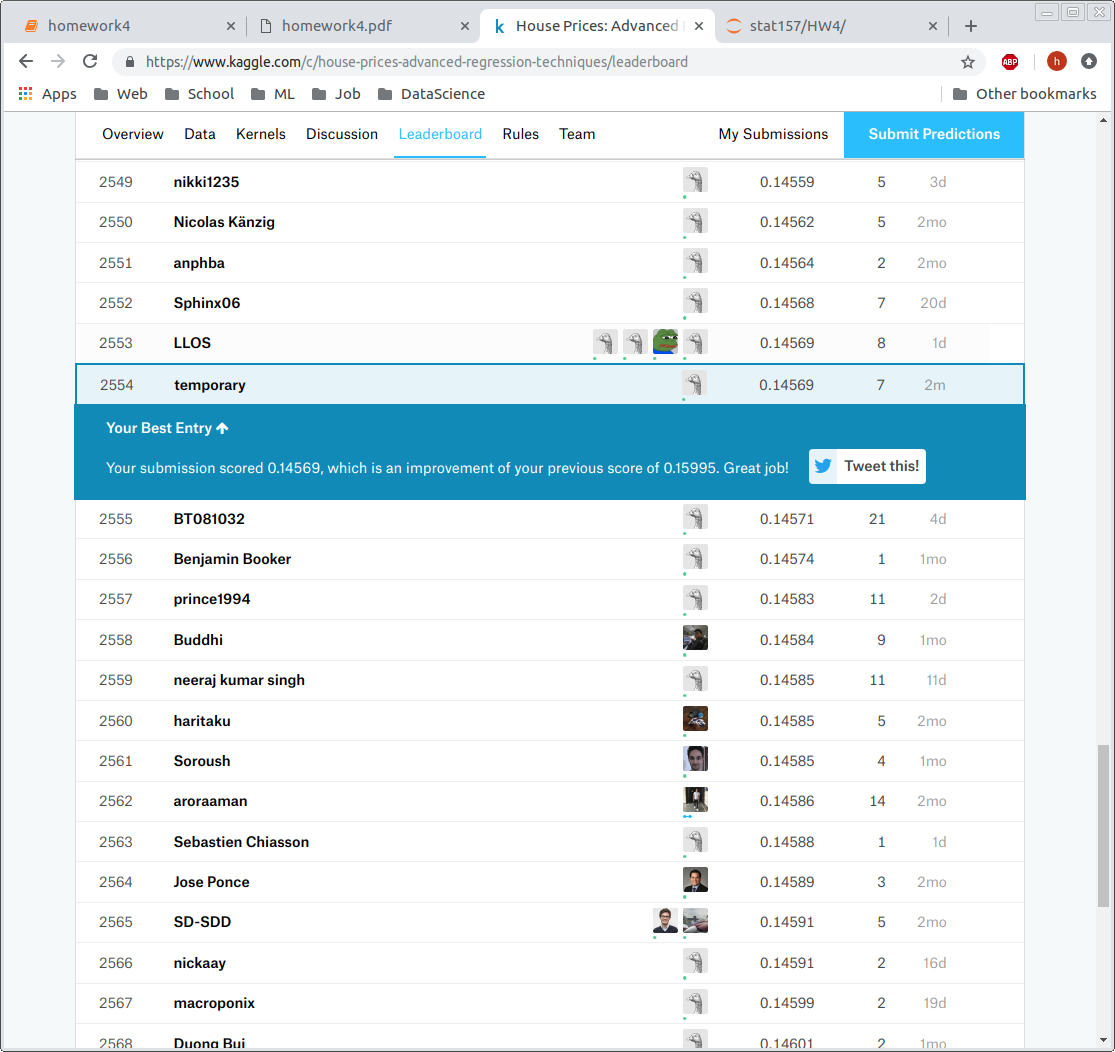
\includegraphics{submission.png}
\caption{submission.png}
\end{figure}

    I had to create a temporary id since the one I used before already
joined this competition with my friends in a group (not from this class
and that was about an year ago) so my username is temporary.

    \begin{Verbatim}[commandchars=\\\{\}]
{\color{incolor}In [{\color{incolor}1}]:} \PY{c+c1}{\PYZsh{} If pandas is not installed, please uncomment the following line:}
        \PY{c+c1}{\PYZsh{} !pip install pandas}
        
        \PY{o}{\PYZpc{}}\PY{k}{matplotlib} inline
        \PY{k+kn}{import} \PY{n+nn}{d2l}
        \PY{k+kn}{from} \PY{n+nn}{mxnet} \PY{k}{import} \PY{n}{autograd}\PY{p}{,} \PY{n}{gluon}\PY{p}{,} \PY{n}{init}\PY{p}{,} \PY{n}{nd}
        \PY{k+kn}{from} \PY{n+nn}{mxnet}\PY{n+nn}{.}\PY{n+nn}{gluon} \PY{k}{import} \PY{n}{data} \PY{k}{as} \PY{n}{gdata}\PY{p}{,} \PY{n}{loss} \PY{k}{as} \PY{n}{gloss}\PY{p}{,} \PY{n}{nn}\PY{p}{,} \PY{n}{utils}
        \PY{k+kn}{import} \PY{n+nn}{numpy} \PY{k}{as} \PY{n+nn}{np}
        \PY{k+kn}{import} \PY{n+nn}{pandas} \PY{k}{as} \PY{n+nn}{pd}
\end{Verbatim}


    We downloaded the data into the current directory. To load the two CSV
(Comma Separated Values) files containing training and test data
respectively we use Pandas.

    \begin{Verbatim}[commandchars=\\\{\}]
{\color{incolor}In [{\color{incolor}2}]:} \PY{c+c1}{\PYZsh{} utils.download(\PYZsq{}https://github.com/d2l\PYZhy{}ai/d2l\PYZhy{}en/raw/master/data/kaggle\PYZus{}house\PYZus{}pred\PYZus{}train.csv\PYZsq{})}
        \PY{c+c1}{\PYZsh{} utils.download(\PYZsq{}https://github.com/d2l\PYZhy{}ai/d2l\PYZhy{}en/raw/master/data/kaggle\PYZus{}house\PYZus{}pred\PYZus{}test.csv\PYZsq{})}
        \PY{n}{train\PYZus{}data} \PY{o}{=} \PY{n}{pd}\PY{o}{.}\PY{n}{read\PYZus{}csv}\PY{p}{(}\PY{l+s+s1}{\PYZsq{}}\PY{l+s+s1}{kaggle\PYZus{}house\PYZus{}pred\PYZus{}train.csv}\PY{l+s+s1}{\PYZsq{}}\PY{p}{)}
        \PY{n}{test\PYZus{}data} \PY{o}{=} \PY{n}{pd}\PY{o}{.}\PY{n}{read\PYZus{}csv}\PY{p}{(}\PY{l+s+s1}{\PYZsq{}}\PY{l+s+s1}{kaggle\PYZus{}house\PYZus{}pred\PYZus{}test.csv}\PY{l+s+s1}{\PYZsq{}}\PY{p}{)}
\end{Verbatim}


    The training data set includes 1,460 examples, 80 features, and 1
label., the test data contains 1,459 examples and 80 features.

    \begin{Verbatim}[commandchars=\\\{\}]
{\color{incolor}In [{\color{incolor}3}]:} \PY{n+nb}{print}\PY{p}{(}\PY{n}{train\PYZus{}data}\PY{o}{.}\PY{n}{shape}\PY{p}{)}
        \PY{n+nb}{print}\PY{p}{(}\PY{n}{test\PYZus{}data}\PY{o}{.}\PY{n}{shape}\PY{p}{)}
\end{Verbatim}


    \begin{Verbatim}[commandchars=\\\{\}]
(1460, 81)
(1459, 80)

    \end{Verbatim}

    Let's take a look at the first 4 and last 2 features as well as the
label (SalePrice) from the first 4 examples:

    \begin{Verbatim}[commandchars=\\\{\}]
{\color{incolor}In [{\color{incolor}4}]:} \PY{n}{train\PYZus{}data}\PY{o}{.}\PY{n}{iloc}\PY{p}{[}\PY{l+m+mi}{0}\PY{p}{:}\PY{l+m+mi}{4}\PY{p}{,} \PY{p}{[}\PY{l+m+mi}{0}\PY{p}{,} \PY{l+m+mi}{1}\PY{p}{,} \PY{l+m+mi}{2}\PY{p}{,} \PY{l+m+mi}{3}\PY{p}{,} \PY{o}{\PYZhy{}}\PY{l+m+mi}{3}\PY{p}{,} \PY{o}{\PYZhy{}}\PY{l+m+mi}{2}\PY{p}{,} \PY{o}{\PYZhy{}}\PY{l+m+mi}{1}\PY{p}{]}\PY{p}{]}
\end{Verbatim}


\begin{Verbatim}[commandchars=\\\{\}]
{\color{outcolor}Out[{\color{outcolor}4}]:}    Id  MSSubClass MSZoning  LotFrontage SaleType SaleCondition  SalePrice
        0   1          60       RL         65.0       WD        Normal     208500
        1   2          20       RL         80.0       WD        Normal     181500
        2   3          60       RL         68.0       WD        Normal     223500
        3   4          70       RL         60.0       WD       Abnorml     140000
\end{Verbatim}
            
    We can see that in each example, the first feature is the ID. This helps
the model identify each training example. While this is convenient, it
doesn't carry any information for prediction purposes. Hence we remove
it from the dataset before feeding the data into the network.

    \begin{Verbatim}[commandchars=\\\{\}]
{\color{incolor}In [{\color{incolor}5}]:} \PY{n}{all\PYZus{}features} \PY{o}{=} \PY{n}{pd}\PY{o}{.}\PY{n}{concat}\PY{p}{(}\PY{p}{(}\PY{n}{train\PYZus{}data}\PY{o}{.}\PY{n}{iloc}\PY{p}{[}\PY{p}{:}\PY{p}{,} \PY{l+m+mi}{1}\PY{p}{:}\PY{o}{\PYZhy{}}\PY{l+m+mi}{1}\PY{p}{]}\PY{p}{,} \PY{n}{test\PYZus{}data}\PY{o}{.}\PY{n}{iloc}\PY{p}{[}\PY{p}{:}\PY{p}{,} \PY{l+m+mi}{1}\PY{p}{:}\PY{p}{]}\PY{p}{)}\PY{p}{)}
\end{Verbatim}


    \hypertarget{data-preprocessing}{%
\subsection{Data Preprocessing}\label{data-preprocessing}}

As stated above, we have a wide variety of datatypes. Before we feed it
into a deep network we need to perform some amount of processing. Let's
start with the numerical features. We begin by replacing missing values
with the mean. This is a reasonable strategy if features are missing at
random. To adjust them to a common scale we rescale them to zero mean
and unit variance. This is accomplished as follows:

\[x \leftarrow \frac{x - \mu}{\sigma}\]

To check that this transforms \(x\) to data with zero mean and unit
variance simply calculate
\(\mathbf{E}[(x-\mu)/\sigma] = (\mu - \mu)/\sigma = 0\). To check the
variance we use \(\mathbf{E}[(x-\mu)^2] = \sigma^2\) and thus the
transformed variable has unit variance. The reason for `normalizing' the
data is that it brings all features to the same order of magnitude.
After all, we do not know \emph{a priori} which features are likely to
be relevant. Hence it makes sense to treat them equally.

    \begin{Verbatim}[commandchars=\\\{\}]
{\color{incolor}In [{\color{incolor}6}]:} \PY{n}{numeric\PYZus{}features} \PY{o}{=} \PY{n}{all\PYZus{}features}\PY{o}{.}\PY{n}{dtypes}\PY{p}{[}\PY{n}{all\PYZus{}features}\PY{o}{.}\PY{n}{dtypes} \PY{o}{!=} \PY{l+s+s1}{\PYZsq{}}\PY{l+s+s1}{object}\PY{l+s+s1}{\PYZsq{}}\PY{p}{]}\PY{o}{.}\PY{n}{index}
        \PY{n}{all\PYZus{}features}\PY{p}{[}\PY{n}{numeric\PYZus{}features}\PY{p}{]} \PY{o}{=} \PY{n}{all\PYZus{}features}\PY{p}{[}\PY{n}{numeric\PYZus{}features}\PY{p}{]}\PY{o}{.}\PY{n}{apply}\PY{p}{(}
            \PY{k}{lambda} \PY{n}{x}\PY{p}{:} \PY{p}{(}\PY{n}{x} \PY{o}{\PYZhy{}} \PY{n}{x}\PY{o}{.}\PY{n}{mean}\PY{p}{(}\PY{p}{)}\PY{p}{)} \PY{o}{/} \PY{p}{(}\PY{n}{x}\PY{o}{.}\PY{n}{std}\PY{p}{(}\PY{p}{)}\PY{p}{)}\PY{p}{)}
        \PY{c+c1}{\PYZsh{} after standardizing the data all means vanish, hence we can set missing values to 0}
        \PY{n}{all\PYZus{}features} \PY{o}{=} \PY{n}{all\PYZus{}features}\PY{o}{.}\PY{n}{fillna}\PY{p}{(}\PY{l+m+mi}{0}\PY{p}{)}
\end{Verbatim}


    Next we deal with discrete values. This includes variables such as
`MSZoning'. We replace them by a one-hot encoding in the same manner as
how we transformed multiclass classification data into a vector of \(0\)
and \(1\). For instance, `MSZoning' assumes the values `RL' and `RM'.
They map into vectors \((1,0)\) and \((0,1)\) respectively. Pandas does
this automatically for us.

    \begin{Verbatim}[commandchars=\\\{\}]
{\color{incolor}In [{\color{incolor}7}]:} \PY{c+c1}{\PYZsh{} Dummy\PYZus{}na=True refers to a missing value being a legal eigenvalue, and creates an indicative feature for it.}
        \PY{n}{all\PYZus{}features} \PY{o}{=} \PY{n}{pd}\PY{o}{.}\PY{n}{get\PYZus{}dummies}\PY{p}{(}\PY{n}{all\PYZus{}features}\PY{p}{,} \PY{n}{dummy\PYZus{}na}\PY{o}{=}\PY{k+kc}{True}\PY{p}{)}
        \PY{n}{all\PYZus{}features}\PY{o}{.}\PY{n}{shape}
\end{Verbatim}


\begin{Verbatim}[commandchars=\\\{\}]
{\color{outcolor}Out[{\color{outcolor}7}]:} (2919, 354)
\end{Verbatim}
            
    You can see that this conversion increases the number of features from
79 to 331. Finally, via the \texttt{values} attribute we can extract the
NumPy format from the Pandas dataframe and convert it into MXNet's
native representation - NDArray for training.

    \begin{Verbatim}[commandchars=\\\{\}]
{\color{incolor}In [{\color{incolor}8}]:} \PY{n}{n\PYZus{}train} \PY{o}{=} \PY{n}{train\PYZus{}data}\PY{o}{.}\PY{n}{shape}\PY{p}{[}\PY{l+m+mi}{0}\PY{p}{]}
        \PY{n}{train\PYZus{}features} \PY{o}{=} \PY{n}{nd}\PY{o}{.}\PY{n}{array}\PY{p}{(}\PY{n}{all\PYZus{}features}\PY{p}{[}\PY{p}{:}\PY{n}{n\PYZus{}train}\PY{p}{]}\PY{o}{.}\PY{n}{values}\PY{p}{)}
        \PY{n}{test\PYZus{}features} \PY{o}{=} \PY{n}{nd}\PY{o}{.}\PY{n}{array}\PY{p}{(}\PY{n}{all\PYZus{}features}\PY{p}{[}\PY{n}{n\PYZus{}train}\PY{p}{:}\PY{p}{]}\PY{o}{.}\PY{n}{values}\PY{p}{)}
        \PY{n}{train\PYZus{}labels} \PY{o}{=} \PY{n}{nd}\PY{o}{.}\PY{n}{array}\PY{p}{(}\PY{n}{train\PYZus{}data}\PY{o}{.}\PY{n}{SalePrice}\PY{o}{.}\PY{n}{values}\PY{p}{)}\PY{o}{.}\PY{n}{reshape}\PY{p}{(}\PY{p}{(}\PY{o}{\PYZhy{}}\PY{l+m+mi}{1}\PY{p}{,} \PY{l+m+mi}{1}\PY{p}{)}\PY{p}{)}
\end{Verbatim}


    \hypertarget{training}{%
\subsection{Training}\label{training}}

To get started we train a linear model with squared loss. This will
obviously not lead to a competition winning submission but it provides a
sanity check to see whether there's meaningful information in the data.
It also amounts to a minimum baseline of how well we should expect any
`fancy' model to work.

    \begin{Verbatim}[commandchars=\\\{\}]
{\color{incolor}In [{\color{incolor}9}]:} \PY{n}{loss} \PY{o}{=} \PY{n}{gloss}\PY{o}{.}\PY{n}{L2Loss}\PY{p}{(}\PY{p}{)}
        
        \PY{k}{def} \PY{n+nf}{get\PYZus{}net}\PY{p}{(}\PY{p}{)}\PY{p}{:}
            \PY{n}{net} \PY{o}{=} \PY{n}{nn}\PY{o}{.}\PY{n}{Sequential}\PY{p}{(}\PY{p}{)}
            \PY{n}{net}\PY{o}{.}\PY{n}{add}\PY{p}{(}\PY{n}{nn}\PY{o}{.}\PY{n}{Dense}\PY{p}{(}\PY{l+m+mi}{80}\PY{p}{,} \PY{n}{activation}\PY{o}{=}\PY{l+s+s1}{\PYZsq{}}\PY{l+s+s1}{relu}\PY{l+s+s1}{\PYZsq{}}\PY{p}{)}\PY{p}{)}
            \PY{n}{net}\PY{o}{.}\PY{n}{add}\PY{p}{(}\PY{n}{nn}\PY{o}{.}\PY{n}{Dropout}\PY{p}{(}\PY{o}{.}\PY{l+m+mi}{5}\PY{p}{)}\PY{p}{)}
            \PY{n}{net}\PY{o}{.}\PY{n}{add}\PY{p}{(}\PY{n}{nn}\PY{o}{.}\PY{n}{BatchNorm}\PY{p}{(}\PY{p}{)}\PY{p}{)}
            \PY{n}{net}\PY{o}{.}\PY{n}{add}\PY{p}{(}\PY{n}{nn}\PY{o}{.}\PY{n}{Dense}\PY{p}{(}\PY{l+m+mi}{20}\PY{p}{,} \PY{n}{activation}\PY{o}{=}\PY{l+s+s1}{\PYZsq{}}\PY{l+s+s1}{relu}\PY{l+s+s1}{\PYZsq{}}\PY{p}{)}\PY{p}{)}
            \PY{n}{net}\PY{o}{.}\PY{n}{add}\PY{p}{(}\PY{n}{nn}\PY{o}{.}\PY{n}{Dropout}\PY{p}{(}\PY{o}{.}\PY{l+m+mi}{5}\PY{p}{)}\PY{p}{)}
            \PY{n}{net}\PY{o}{.}\PY{n}{add}\PY{p}{(}\PY{n}{nn}\PY{o}{.}\PY{n}{BatchNorm}\PY{p}{(}\PY{p}{)}\PY{p}{)}
            \PY{n}{net}\PY{o}{.}\PY{n}{add}\PY{p}{(}\PY{n}{nn}\PY{o}{.}\PY{n}{Dense}\PY{p}{(}\PY{l+m+mi}{1}\PY{p}{)}\PY{p}{)}
            \PY{n}{net}\PY{o}{.}\PY{n}{initialize}\PY{p}{(}\PY{n}{init}\PY{o}{=}\PY{n}{init}\PY{o}{.}\PY{n}{Xavier}\PY{p}{(}\PY{p}{)}\PY{p}{)}
            \PY{k}{return} \PY{n}{net}
\end{Verbatim}


    House prices, like shares, are relative. That is, we probably care more
about the relative error \(\frac{y - \hat{y}}{y}\) than about the
absolute error. For instance, getting a house price wrong by USD 100,000
is terrible in Rural Ohio, where the value of the house is USD 125,000.
On the other hand, if we err by this amount in Los Altos Hills,
California, we can be proud of the accuracy of our model (the median
house price there exceeds 4 million).

One way to address this problem is to measure the discrepancy in the
logarithm of the price estimates. In fact, this is also the error that
is being used to measure the quality in this competition. After all, a
small value \(\delta\) of \(\log y - \log \hat{y}\) translates into
\(e^{-\delta} \leq \frac{\hat{y}}{y} \leq e^\delta\). This leads to the
following loss function:

\[L = \sqrt{\frac{1}{n}\sum_{i=1}^n\left(\log y_i -\log \hat{y}_i\right)^2}\]

    \begin{Verbatim}[commandchars=\\\{\}]
{\color{incolor}In [{\color{incolor}10}]:} \PY{k}{def} \PY{n+nf}{log\PYZus{}rmse}\PY{p}{(}\PY{n}{net}\PY{p}{,} \PY{n}{features}\PY{p}{,} \PY{n}{labels}\PY{p}{)}\PY{p}{:}
             \PY{c+c1}{\PYZsh{} To further stabilize the value when the logarithm is taken, set the value less than 1 as 1.}
             \PY{n}{clipped\PYZus{}preds} \PY{o}{=} \PY{n}{nd}\PY{o}{.}\PY{n}{clip}\PY{p}{(}\PY{n}{net}\PY{p}{(}\PY{n}{features}\PY{p}{)}\PY{p}{,} \PY{l+m+mi}{1}\PY{p}{,} \PY{n+nb}{float}\PY{p}{(}\PY{l+s+s1}{\PYZsq{}}\PY{l+s+s1}{inf}\PY{l+s+s1}{\PYZsq{}}\PY{p}{)}\PY{p}{)}
             \PY{n}{rmse} \PY{o}{=} \PY{n}{nd}\PY{o}{.}\PY{n}{sqrt}\PY{p}{(}\PY{l+m+mi}{2} \PY{o}{*} \PY{n}{loss}\PY{p}{(}\PY{n}{clipped\PYZus{}preds}\PY{o}{.}\PY{n}{log}\PY{p}{(}\PY{p}{)}\PY{p}{,} \PY{n}{labels}\PY{o}{.}\PY{n}{log}\PY{p}{(}\PY{p}{)}\PY{p}{)}\PY{o}{.}\PY{n}{mean}\PY{p}{(}\PY{p}{)}\PY{p}{)}
             \PY{k}{return} \PY{n}{rmse}\PY{o}{.}\PY{n}{asscalar}\PY{p}{(}\PY{p}{)}
\end{Verbatim}


    Unlike in the previous sections, the following training functions use
the Adam optimization algorithm. Compared to the previously used
mini-batch stochastic gradient descent, the Adam optimization algorithm
is relatively less sensitive to learning rates. This will be covered in
further detail later on when we discuss the details on
\href{../chapter_optimization/index.md}{Optimization Algorithms} in a
separate chapter.

    \begin{Verbatim}[commandchars=\\\{\}]
{\color{incolor}In [{\color{incolor}11}]:} \PY{k}{def} \PY{n+nf}{train}\PY{p}{(}\PY{n}{net}\PY{p}{,} \PY{n}{train\PYZus{}features}\PY{p}{,} \PY{n}{train\PYZus{}labels}\PY{p}{,} \PY{n}{test\PYZus{}features}\PY{p}{,} \PY{n}{test\PYZus{}labels}\PY{p}{,}
                   \PY{n}{num\PYZus{}epochs}\PY{p}{,} \PY{n}{learning\PYZus{}rate}\PY{p}{,} \PY{n}{weight\PYZus{}decay}\PY{p}{,} \PY{n}{batch\PYZus{}size}\PY{p}{)}\PY{p}{:}
             \PY{n}{train\PYZus{}ls}\PY{p}{,} \PY{n}{test\PYZus{}ls} \PY{o}{=} \PY{p}{[}\PY{p}{]}\PY{p}{,} \PY{p}{[}\PY{p}{]}
             \PY{n}{train\PYZus{}iter} \PY{o}{=} \PY{n}{gdata}\PY{o}{.}\PY{n}{DataLoader}\PY{p}{(}\PY{n}{gdata}\PY{o}{.}\PY{n}{ArrayDataset}\PY{p}{(}
                 \PY{n}{train\PYZus{}features}\PY{p}{,} \PY{n}{train\PYZus{}labels}\PY{p}{)}\PY{p}{,} \PY{n}{batch\PYZus{}size}\PY{p}{,} \PY{n}{shuffle}\PY{o}{=}\PY{k+kc}{True}\PY{p}{)}
             \PY{c+c1}{\PYZsh{} The Adam optimization algorithm is used here.}
             \PY{n}{trainer} \PY{o}{=} \PY{n}{gluon}\PY{o}{.}\PY{n}{Trainer}\PY{p}{(}\PY{n}{net}\PY{o}{.}\PY{n}{collect\PYZus{}params}\PY{p}{(}\PY{p}{)}\PY{p}{,} \PY{l+s+s1}{\PYZsq{}}\PY{l+s+s1}{adam}\PY{l+s+s1}{\PYZsq{}}\PY{p}{,} \PY{p}{\PYZob{}}
                 \PY{l+s+s1}{\PYZsq{}}\PY{l+s+s1}{learning\PYZus{}rate}\PY{l+s+s1}{\PYZsq{}}\PY{p}{:} \PY{n}{learning\PYZus{}rate}\PY{p}{,} \PY{l+s+s1}{\PYZsq{}}\PY{l+s+s1}{wd}\PY{l+s+s1}{\PYZsq{}}\PY{p}{:} \PY{n}{weight\PYZus{}decay}\PY{p}{\PYZcb{}}\PY{p}{)}
             \PY{k}{for} \PY{n}{epoch} \PY{o+ow}{in} \PY{n+nb}{range}\PY{p}{(}\PY{n}{num\PYZus{}epochs}\PY{p}{)}\PY{p}{:}
                 \PY{k}{for} \PY{n}{X}\PY{p}{,} \PY{n}{y} \PY{o+ow}{in} \PY{n}{train\PYZus{}iter}\PY{p}{:}
                     \PY{k}{with} \PY{n}{autograd}\PY{o}{.}\PY{n}{record}\PY{p}{(}\PY{p}{)}\PY{p}{:}
                         \PY{n}{l} \PY{o}{=} \PY{n}{loss}\PY{p}{(}\PY{n}{net}\PY{p}{(}\PY{n}{X}\PY{p}{)}\PY{p}{,} \PY{n}{y}\PY{p}{)}
                     \PY{n}{l}\PY{o}{.}\PY{n}{backward}\PY{p}{(}\PY{p}{)}
                     \PY{n}{trainer}\PY{o}{.}\PY{n}{step}\PY{p}{(}\PY{n}{batch\PYZus{}size}\PY{p}{)}
                 \PY{n}{train\PYZus{}ls}\PY{o}{.}\PY{n}{append}\PY{p}{(}\PY{n}{log\PYZus{}rmse}\PY{p}{(}\PY{n}{net}\PY{p}{,} \PY{n}{train\PYZus{}features}\PY{p}{,} \PY{n}{train\PYZus{}labels}\PY{p}{)}\PY{p}{)}
                 \PY{k}{if} \PY{n}{test\PYZus{}labels} \PY{o+ow}{is} \PY{o+ow}{not} \PY{k+kc}{None}\PY{p}{:}
                     \PY{n}{test\PYZus{}ls}\PY{o}{.}\PY{n}{append}\PY{p}{(}\PY{n}{log\PYZus{}rmse}\PY{p}{(}\PY{n}{net}\PY{p}{,} \PY{n}{test\PYZus{}features}\PY{p}{,} \PY{n}{test\PYZus{}labels}\PY{p}{)}\PY{p}{)}
             \PY{k}{return} \PY{n}{train\PYZus{}ls}\PY{p}{,} \PY{n}{test\PYZus{}ls}
\end{Verbatim}


    \hypertarget{k-fold-cross-validation}{%
\subsection{k-Fold Cross-Validation}\label{k-fold-cross-validation}}

The k-fold cross-validation was introduced in the section where we
discussed how to deal with \href{underfit-overfit.md}{``Model Selection,
Underfitting and Overfitting''}. We will put this to good use to select
the model design and to adjust the hyperparameters. We first need a
function that returns the i-th fold of the data in a k-fold
cros-validation procedure. It proceeds by slicing out the i-th segment
as validation data and returning the rest as training data. Note - this
is not the most efficient way of handling data and we would use
something much smarter if the amount of data was considerably larger.
But this would obscure the function of the code considerably and we thus
omit it.

    \begin{Verbatim}[commandchars=\\\{\}]
{\color{incolor}In [{\color{incolor}12}]:} \PY{k}{def} \PY{n+nf}{get\PYZus{}k\PYZus{}fold\PYZus{}data}\PY{p}{(}\PY{n}{k}\PY{p}{,} \PY{n}{i}\PY{p}{,} \PY{n}{X}\PY{p}{,} \PY{n}{y}\PY{p}{)}\PY{p}{:}
             \PY{k}{assert} \PY{n}{k} \PY{o}{\PYZgt{}} \PY{l+m+mi}{1}
             \PY{n}{fold\PYZus{}size} \PY{o}{=} \PY{n}{X}\PY{o}{.}\PY{n}{shape}\PY{p}{[}\PY{l+m+mi}{0}\PY{p}{]} \PY{o}{/}\PY{o}{/} \PY{n}{k}
             \PY{n}{X\PYZus{}train}\PY{p}{,} \PY{n}{y\PYZus{}train} \PY{o}{=} \PY{k+kc}{None}\PY{p}{,} \PY{k+kc}{None}
             \PY{k}{for} \PY{n}{j} \PY{o+ow}{in} \PY{n+nb}{range}\PY{p}{(}\PY{n}{k}\PY{p}{)}\PY{p}{:}
                 \PY{n}{idx} \PY{o}{=} \PY{n+nb}{slice}\PY{p}{(}\PY{n}{j} \PY{o}{*} \PY{n}{fold\PYZus{}size}\PY{p}{,} \PY{p}{(}\PY{n}{j} \PY{o}{+} \PY{l+m+mi}{1}\PY{p}{)} \PY{o}{*} \PY{n}{fold\PYZus{}size}\PY{p}{)}
                 \PY{n}{X\PYZus{}part}\PY{p}{,} \PY{n}{y\PYZus{}part} \PY{o}{=} \PY{n}{X}\PY{p}{[}\PY{n}{idx}\PY{p}{,} \PY{p}{:}\PY{p}{]}\PY{p}{,} \PY{n}{y}\PY{p}{[}\PY{n}{idx}\PY{p}{]}
                 \PY{k}{if} \PY{n}{j} \PY{o}{==} \PY{n}{i}\PY{p}{:}
                     \PY{n}{X\PYZus{}valid}\PY{p}{,} \PY{n}{y\PYZus{}valid} \PY{o}{=} \PY{n}{X\PYZus{}part}\PY{p}{,} \PY{n}{y\PYZus{}part}
                 \PY{k}{elif} \PY{n}{X\PYZus{}train} \PY{o+ow}{is} \PY{k+kc}{None}\PY{p}{:}
                     \PY{n}{X\PYZus{}train}\PY{p}{,} \PY{n}{y\PYZus{}train} \PY{o}{=} \PY{n}{X\PYZus{}part}\PY{p}{,} \PY{n}{y\PYZus{}part}
                 \PY{k}{else}\PY{p}{:}
                     \PY{n}{X\PYZus{}train} \PY{o}{=} \PY{n}{nd}\PY{o}{.}\PY{n}{concat}\PY{p}{(}\PY{n}{X\PYZus{}train}\PY{p}{,} \PY{n}{X\PYZus{}part}\PY{p}{,} \PY{n}{dim}\PY{o}{=}\PY{l+m+mi}{0}\PY{p}{)}
                     \PY{n}{y\PYZus{}train} \PY{o}{=} \PY{n}{nd}\PY{o}{.}\PY{n}{concat}\PY{p}{(}\PY{n}{y\PYZus{}train}\PY{p}{,} \PY{n}{y\PYZus{}part}\PY{p}{,} \PY{n}{dim}\PY{o}{=}\PY{l+m+mi}{0}\PY{p}{)}
             \PY{k}{return} \PY{n}{X\PYZus{}train}\PY{p}{,} \PY{n}{y\PYZus{}train}\PY{p}{,} \PY{n}{X\PYZus{}valid}\PY{p}{,} \PY{n}{y\PYZus{}valid}
\end{Verbatim}


    The training and verification error averages are returned when we train
\(k\) times in the k-fold cross-validation.

    \begin{Verbatim}[commandchars=\\\{\}]
{\color{incolor}In [{\color{incolor}13}]:} \PY{k}{def} \PY{n+nf}{k\PYZus{}fold}\PY{p}{(}\PY{n}{k}\PY{p}{,} \PY{n}{X\PYZus{}train}\PY{p}{,} \PY{n}{y\PYZus{}train}\PY{p}{,} \PY{n}{num\PYZus{}epochs}\PY{p}{,}
                    \PY{n}{learning\PYZus{}rate}\PY{p}{,} \PY{n}{weight\PYZus{}decay}\PY{p}{,} \PY{n}{batch\PYZus{}size}\PY{p}{)}\PY{p}{:}
             \PY{n}{train\PYZus{}l\PYZus{}sum}\PY{p}{,} \PY{n}{valid\PYZus{}l\PYZus{}sum} \PY{o}{=} \PY{l+m+mi}{0}\PY{p}{,} \PY{l+m+mi}{0}
             \PY{k}{for} \PY{n}{i} \PY{o+ow}{in} \PY{n+nb}{range}\PY{p}{(}\PY{n}{k}\PY{p}{)}\PY{p}{:}
                 \PY{n}{data} \PY{o}{=} \PY{n}{get\PYZus{}k\PYZus{}fold\PYZus{}data}\PY{p}{(}\PY{n}{k}\PY{p}{,} \PY{n}{i}\PY{p}{,} \PY{n}{X\PYZus{}train}\PY{p}{,} \PY{n}{y\PYZus{}train}\PY{p}{)}
                 \PY{n}{net} \PY{o}{=} \PY{n}{get\PYZus{}net}\PY{p}{(}\PY{p}{)}
                 
                 \PY{n}{train\PYZus{}ls}\PY{p}{,} \PY{n}{valid\PYZus{}ls} \PY{o}{=} \PY{n}{train}\PY{p}{(}\PY{n}{net}\PY{p}{,} \PY{o}{*}\PY{n}{data}\PY{p}{,} \PY{n}{num\PYZus{}epochs}\PY{p}{,} \PY{n}{learning\PYZus{}rate}\PY{p}{,}
                                            \PY{n}{weight\PYZus{}decay}\PY{p}{,} \PY{n}{batch\PYZus{}size}\PY{p}{)}
                 \PY{n}{train\PYZus{}l\PYZus{}sum} \PY{o}{+}\PY{o}{=} \PY{n}{train\PYZus{}ls}\PY{p}{[}\PY{o}{\PYZhy{}}\PY{l+m+mi}{1}\PY{p}{]}
                 \PY{n}{valid\PYZus{}l\PYZus{}sum} \PY{o}{+}\PY{o}{=} \PY{n}{valid\PYZus{}ls}\PY{p}{[}\PY{o}{\PYZhy{}}\PY{l+m+mi}{1}\PY{p}{]}
         \PY{c+c1}{\PYZsh{}         if i == 0:}
         \PY{c+c1}{\PYZsh{}             d2l.semilogy(range(1, num\PYZus{}epochs + 1), train\PYZus{}ls, \PYZsq{}epochs\PYZsq{}, \PYZsq{}rmse\PYZsq{},}
         \PY{c+c1}{\PYZsh{}                         range(1, num\PYZus{}epochs + 1), valid\PYZus{}ls,}
         \PY{c+c1}{\PYZsh{}                         [\PYZsq{}train\PYZsq{}, \PYZsq{}valid\PYZsq{}])}
         \PY{c+c1}{\PYZsh{}         print(\PYZsq{}fold \PYZpc{}d, train rmse: \PYZpc{}f, valid rmse: \PYZpc{}f\PYZsq{} \PYZpc{} (}
         \PY{c+c1}{\PYZsh{}             i, train\PYZus{}ls[\PYZhy{}1], valid\PYZus{}ls[\PYZhy{}1]))}
             \PY{k}{return} \PY{n}{net}\PY{p}{,} \PY{n}{train\PYZus{}l\PYZus{}sum} \PY{o}{/} \PY{n}{k}\PY{p}{,} \PY{n}{valid\PYZus{}l\PYZus{}sum} \PY{o}{/} \PY{n}{k}
\end{Verbatim}


    \hypertarget{model-selection}{%
\subsection{Model Selection}\label{model-selection}}

We pick a rather un-tuned set of hyperparameters and leave it up to the
reader to improve the model considerably. Finding a good choice can take
quite some time, depending on how many things one wants to optimize
over. Within reason the k-fold crossvalidation approach is resilient
against multiple testing. However, if we were to try out an unreasonably
large number of options it might fail since we might just get lucky on
the validation split with a particular set of hyperparameters.

    \hypertarget{custom-preprocessing}{%
\subsubsection{Custom Preprocessing}\label{custom-preprocessing}}

    \begin{Verbatim}[commandchars=\\\{\}]
{\color{incolor}In [{\color{incolor}14}]:} \PY{k+kn}{from} \PY{n+nn}{sklearn}\PY{n+nn}{.}\PY{n+nn}{cross\PYZus{}decomposition} \PY{k}{import} \PY{n}{CCA}
         \PY{k+kn}{import} \PY{n+nn}{matplotlib}\PY{n+nn}{.}\PY{n+nn}{pyplot} \PY{k}{as} \PY{n+nn}{plt}
         \PY{k+kn}{from} \PY{n+nn}{sklearn}\PY{n+nn}{.}\PY{n+nn}{preprocessing} \PY{k}{import} \PY{n}{normalize}
         \PY{k+kn}{from} \PY{n+nn}{sklearn}\PY{n+nn}{.}\PY{n+nn}{model\PYZus{}selection} \PY{k}{import} \PY{n}{train\PYZus{}test\PYZus{}split}
         \PY{k+kn}{from} \PY{n+nn}{sklearn}\PY{n+nn}{.}\PY{n+nn}{metrics} \PY{k}{import} \PY{n}{r2\PYZus{}score}
         \PY{k+kn}{import} \PY{n+nn}{xgboost}
\end{Verbatim}


    \begin{Verbatim}[commandchars=\\\{\}]
{\color{incolor}In [{\color{incolor}15}]:} \PY{k}{def} \PY{n+nf}{check}\PY{p}{(}\PY{n}{X\PYZus{}train}\PY{p}{,} \PY{n}{y\PYZus{}train}\PY{p}{)}\PY{p}{:}
             \PY{n}{xgb} \PY{o}{=} \PY{n}{xgboost}\PY{o}{.}\PY{n}{XGBRegressor}\PY{p}{(}\PY{n}{n\PYZus{}estimators}\PY{o}{=}\PY{l+m+mi}{100}\PY{p}{,} \PY{n}{learning\PYZus{}rate}\PY{o}{=}\PY{l+m+mf}{0.08}\PY{p}{,} \PY{n}{gamma}\PY{o}{=}\PY{l+m+mi}{0}\PY{p}{,} \PY{n}{subsample}\PY{o}{=}\PY{l+m+mf}{0.75}\PY{p}{,}
                                        \PY{n}{colsample\PYZus{}bytree}\PY{o}{=}\PY{l+m+mi}{1}\PY{p}{,} \PY{n}{max\PYZus{}depth}\PY{o}{=}\PY{l+m+mi}{7}\PY{p}{)}
         
             \PY{n}{X\PYZus{}train}\PY{p}{,} \PY{n}{X\PYZus{}test}\PY{p}{,} \PY{n}{y\PYZus{}train}\PY{p}{,} \PY{n}{y\PYZus{}test} \PY{o}{=} \PY{n}{train\PYZus{}test\PYZus{}split}\PY{p}{(}\PY{n}{X\PYZus{}train}\PY{p}{,} \PY{n}{y\PYZus{}train}\PY{p}{)}
         
             \PY{n}{xgb}\PY{o}{.}\PY{n}{fit}\PY{p}{(}\PY{n}{X\PYZus{}train}\PY{p}{,} \PY{n}{y\PYZus{}train}\PY{p}{)}
             \PY{n}{pred} \PY{o}{=} \PY{n}{xgb}\PY{o}{.}\PY{n}{predict}\PY{p}{(}\PY{n}{X\PYZus{}test}\PY{p}{)}
             \PY{n+nb}{print}\PY{p}{(}\PY{l+s+s1}{\PYZsq{}}\PY{l+s+s1}{xgb:}\PY{l+s+s1}{\PYZsq{}}\PY{p}{,} \PY{n}{r2\PYZus{}score}\PY{p}{(}\PY{n}{y\PYZus{}test}\PY{p}{,} \PY{n}{pred}\PY{p}{)}\PY{p}{)}
             
             \PY{k}{return} \PY{n}{xgb}
             
         \PY{k}{def} \PY{n+nf}{preprocess}\PY{p}{(}\PY{n}{dat}\PY{p}{,} \PY{n}{test}\PY{o}{=}\PY{k+kc}{False}\PY{p}{,} \PY{n}{obj\PYZus{}features}\PY{o}{=}\PY{k+kc}{None}\PY{p}{,} \PY{n}{num\PYZus{}features}\PY{o}{=}\PY{k+kc}{None}\PY{p}{)}\PY{p}{:}
         
             \PY{n}{data} \PY{o}{=} \PY{n}{dat}\PY{o}{.}\PY{n}{copy}\PY{p}{(}\PY{p}{)}
         
             \PY{k}{if} \PY{o+ow}{not} \PY{n}{test}\PY{p}{:}
                 \PY{n}{data} \PY{o}{=} \PY{n}{data}\PY{p}{[}\PY{n}{data}\PY{p}{[}\PY{l+s+s1}{\PYZsq{}}\PY{l+s+s1}{SalePrice}\PY{l+s+s1}{\PYZsq{}}\PY{p}{]} \PY{o}{\PYZlt{}} \PY{n}{data}\PY{p}{[}\PY{l+s+s1}{\PYZsq{}}\PY{l+s+s1}{SalePrice}\PY{l+s+s1}{\PYZsq{}}\PY{p}{]}\PY{o}{.}\PY{n}{quantile}\PY{p}{(}\PY{o}{.}\PY{l+m+mi}{95}\PY{p}{)}\PY{p}{]}
                 \PY{n}{data} \PY{o}{=} \PY{n}{data}\PY{p}{[}\PY{n}{data}\PY{p}{[}\PY{l+s+s1}{\PYZsq{}}\PY{l+s+s1}{1stFlrSF}\PY{l+s+s1}{\PYZsq{}}\PY{p}{]} \PY{o}{\PYZlt{}} \PY{n}{data}\PY{p}{[}\PY{l+s+s1}{\PYZsq{}}\PY{l+s+s1}{1stFlrSF}\PY{l+s+s1}{\PYZsq{}}\PY{p}{]}\PY{o}{.}\PY{n}{quantile}\PY{p}{(}\PY{o}{.}\PY{l+m+mi}{95}\PY{p}{)}\PY{p}{]}
                 \PY{n}{data} \PY{o}{=} \PY{n}{data}\PY{p}{[}\PY{n}{data}\PY{p}{[}\PY{l+s+s1}{\PYZsq{}}\PY{l+s+s1}{LotArea}\PY{l+s+s1}{\PYZsq{}}\PY{p}{]} \PY{o}{\PYZlt{}} \PY{n}{data}\PY{p}{[}\PY{l+s+s1}{\PYZsq{}}\PY{l+s+s1}{LotArea}\PY{l+s+s1}{\PYZsq{}}\PY{p}{]}\PY{o}{.}\PY{n}{quantile}\PY{p}{(}\PY{o}{.}\PY{l+m+mi}{95}\PY{p}{)}\PY{p}{]}
         
             \PY{n}{data} \PY{o}{=} \PY{n}{data}\PY{p}{[}\PY{n}{data}\PY{o}{.}\PY{n}{dtypes}\PY{p}{[}\PY{n}{data}\PY{o}{.}\PY{n}{dtypes} \PY{o}{!=} \PY{l+s+s1}{\PYZsq{}}\PY{l+s+s1}{object}\PY{l+s+s1}{\PYZsq{}}\PY{p}{]}\PY{o}{.}\PY{n}{index}\PY{p}{]}
             
         
             \PY{k}{if} \PY{n}{obj\PYZus{}features} \PY{o+ow}{is} \PY{o+ow}{not} \PY{k+kc}{None}\PY{p}{:}
                 \PY{k}{if} \PY{o+ow}{not} \PY{n}{test}\PY{p}{:}
                     \PY{n}{data} \PY{o}{=} \PY{n}{pd}\PY{o}{.}\PY{n}{concat}\PY{p}{(}\PY{p}{[}\PY{n}{data}\PY{p}{,} \PY{n}{train\PYZus{}data}\PY{o}{.}\PY{n}{iloc}\PY{p}{[}\PY{n}{data}\PY{o}{.}\PY{n}{index}\PY{p}{]}\PY{p}{[}\PY{n}{obj\PYZus{}features}\PY{p}{]}\PY{p}{]}\PY{p}{,} \PY{n}{axis}\PY{o}{=}\PY{l+m+mi}{1}\PY{p}{)}
                 \PY{k}{else}\PY{p}{:}
                     \PY{n}{data} \PY{o}{=} \PY{n}{pd}\PY{o}{.}\PY{n}{concat}\PY{p}{(}\PY{p}{[}\PY{n}{data}\PY{p}{,} \PY{n}{test\PYZus{}data}\PY{o}{.}\PY{n}{iloc}\PY{p}{[}\PY{n}{data}\PY{o}{.}\PY{n}{index}\PY{p}{]}\PY{p}{[}\PY{n}{obj\PYZus{}features}\PY{p}{]}\PY{p}{]}\PY{p}{,} \PY{n}{axis}\PY{o}{=}\PY{l+m+mi}{1}\PY{p}{)}
         
             \PY{n}{data}\PY{p}{[}\PY{l+s+s1}{\PYZsq{}}\PY{l+s+s1}{Bath}\PY{l+s+s1}{\PYZsq{}}\PY{p}{]} \PY{o}{=} \PY{n}{data}\PY{p}{[}\PY{l+s+s1}{\PYZsq{}}\PY{l+s+s1}{FullBath}\PY{l+s+s1}{\PYZsq{}}\PY{p}{]} \PY{o}{+} \PY{p}{(}\PY{l+m+mf}{0.5} \PY{o}{*} \PY{n}{data}\PY{p}{[}\PY{l+s+s1}{\PYZsq{}}\PY{l+s+s1}{HalfBath}\PY{l+s+s1}{\PYZsq{}}\PY{p}{]}\PY{p}{)}
             \PY{n}{data}\PY{p}{[}\PY{l+s+s1}{\PYZsq{}}\PY{l+s+s1}{BsmtBath}\PY{l+s+s1}{\PYZsq{}}\PY{p}{]} \PY{o}{=} \PY{n}{data}\PY{p}{[}\PY{l+s+s1}{\PYZsq{}}\PY{l+s+s1}{BsmtFullBath}\PY{l+s+s1}{\PYZsq{}}\PY{p}{]} \PY{o}{+} \PY{p}{(}\PY{l+m+mf}{0.5} \PY{o}{*} \PY{n}{data}\PY{p}{[}\PY{l+s+s1}{\PYZsq{}}\PY{l+s+s1}{BsmtHalfBath}\PY{l+s+s1}{\PYZsq{}}\PY{p}{]}\PY{p}{)}
         
             \PY{n}{data}\PY{p}{[}\PY{l+s+s1}{\PYZsq{}}\PY{l+s+s1}{TotalFlrSF}\PY{l+s+s1}{\PYZsq{}}\PY{p}{]} \PY{o}{=} \PY{n}{data}\PY{p}{[}\PY{l+s+s1}{\PYZsq{}}\PY{l+s+s1}{1stFlrSF}\PY{l+s+s1}{\PYZsq{}}\PY{p}{]} \PY{o}{+} \PY{p}{(}\PY{l+m+mf}{0.75} \PY{o}{*} \PY{n}{data}\PY{p}{[}\PY{l+s+s1}{\PYZsq{}}\PY{l+s+s1}{2ndFlrSF}\PY{l+s+s1}{\PYZsq{}}\PY{p}{]}\PY{p}{)}
             \PY{n}{data} \PY{o}{=} \PY{n}{data}\PY{o}{.}\PY{n}{drop}\PY{p}{(}\PY{p}{[}\PY{l+s+s1}{\PYZsq{}}\PY{l+s+s1}{1stFlrSF}\PY{l+s+s1}{\PYZsq{}}\PY{p}{,} \PY{l+s+s1}{\PYZsq{}}\PY{l+s+s1}{2ndFlrSF}\PY{l+s+s1}{\PYZsq{}}\PY{p}{]}\PY{p}{,} \PY{n}{axis}\PY{o}{=}\PY{l+m+mi}{1}\PY{p}{)}
             
             \PY{k}{if} \PY{n}{num\PYZus{}features} \PY{o+ow}{is} \PY{o+ow}{not} \PY{k+kc}{None}\PY{p}{:}
                 \PY{n}{data} \PY{o}{=} \PY{n}{data}\PY{o}{.}\PY{n}{drop}\PY{p}{(}\PY{n}{num\PYZus{}features}\PY{p}{,} \PY{n}{axis}\PY{o}{=}\PY{l+m+mi}{1}\PY{p}{)}
             
             \PY{c+c1}{\PYZsh{} id for test data}
             \PY{n}{ids} \PY{o}{=} \PY{k+kc}{None}
             
             \PY{k}{if} \PY{n}{test}\PY{p}{:}
                 \PY{n}{ids} \PY{o}{=} \PY{n}{data}\PY{p}{[}\PY{l+s+s1}{\PYZsq{}}\PY{l+s+s1}{Id}\PY{l+s+s1}{\PYZsq{}}\PY{p}{]}
                 
             \PY{n}{data} \PY{o}{=} \PY{n}{data}\PY{o}{.}\PY{n}{drop}\PY{p}{(}\PY{p}{[}\PY{l+s+s1}{\PYZsq{}}\PY{l+s+s1}{FullBath}\PY{l+s+s1}{\PYZsq{}}\PY{p}{,} \PY{l+s+s1}{\PYZsq{}}\PY{l+s+s1}{HalfBath}\PY{l+s+s1}{\PYZsq{}}\PY{p}{,} \PY{l+s+s1}{\PYZsq{}}\PY{l+s+s1}{BsmtFullBath}\PY{l+s+s1}{\PYZsq{}}\PY{p}{,} \PY{l+s+s1}{\PYZsq{}}\PY{l+s+s1}{BsmtHalfBath}\PY{l+s+s1}{\PYZsq{}}\PY{p}{,} \PY{l+s+s1}{\PYZsq{}}\PY{l+s+s1}{Id}\PY{l+s+s1}{\PYZsq{}}\PY{p}{,} \PY{l+s+s1}{\PYZsq{}}\PY{l+s+s1}{MiscVal}\PY{l+s+s1}{\PYZsq{}}\PY{p}{]}\PY{p}{,} \PY{n}{axis}\PY{o}{=}\PY{l+m+mi}{1}\PY{p}{)}
             
             \PY{k}{return} \PY{n}{data}\PY{p}{,} \PY{n}{ids}
\end{Verbatim}


    \begin{Verbatim}[commandchars=\\\{\}]
{\color{incolor}In [{\color{incolor}16}]:} \PY{n}{train\PYZus{}data} \PY{o}{=} \PY{n}{pd}\PY{o}{.}\PY{n}{read\PYZus{}csv}\PY{p}{(}\PY{l+s+s1}{\PYZsq{}}\PY{l+s+s1}{kaggle\PYZus{}house\PYZus{}pred\PYZus{}train.csv}\PY{l+s+s1}{\PYZsq{}}\PY{p}{)}
         \PY{n}{test\PYZus{}data} \PY{o}{=} \PY{n}{pd}\PY{o}{.}\PY{n}{read\PYZus{}csv}\PY{p}{(}\PY{l+s+s1}{\PYZsq{}}\PY{l+s+s1}{kaggle\PYZus{}house\PYZus{}pred\PYZus{}test.csv}\PY{l+s+s1}{\PYZsq{}}\PY{p}{)}
         
         \PY{n}{obj\PYZus{}features} \PY{o}{=} \PY{p}{[}\PY{l+s+s1}{\PYZsq{}}\PY{l+s+s1}{SaleCondition}\PY{l+s+s1}{\PYZsq{}}\PY{p}{,} \PY{l+s+s1}{\PYZsq{}}\PY{l+s+s1}{MSZoning}\PY{l+s+s1}{\PYZsq{}}\PY{p}{,} \PY{l+s+s1}{\PYZsq{}}\PY{l+s+s1}{BldgType}\PY{l+s+s1}{\PYZsq{}}\PY{p}{,} \PY{l+s+s1}{\PYZsq{}}\PY{l+s+s1}{Neighborhood}\PY{l+s+s1}{\PYZsq{}}\PY{p}{,} \PY{l+s+s1}{\PYZsq{}}\PY{l+s+s1}{LotConfig}\PY{l+s+s1}{\PYZsq{}}\PY{p}{]}
         \PY{n}{num\PYZus{}features} \PY{o}{=} \PY{p}{[}\PY{l+s+s1}{\PYZsq{}}\PY{l+s+s1}{GarageCars}\PY{l+s+s1}{\PYZsq{}}\PY{p}{,} \PY{l+s+s1}{\PYZsq{}}\PY{l+s+s1}{Fireplaces}\PY{l+s+s1}{\PYZsq{}}\PY{p}{,} \PY{l+s+s1}{\PYZsq{}}\PY{l+s+s1}{MSSubClass}\PY{l+s+s1}{\PYZsq{}}\PY{p}{,} \PY{l+s+s1}{\PYZsq{}}\PY{l+s+s1}{LotFrontage}\PY{l+s+s1}{\PYZsq{}}\PY{p}{,} \PY{l+s+s1}{\PYZsq{}}\PY{l+s+s1}{LotArea}\PY{l+s+s1}{\PYZsq{}}\PY{p}{,} \PY{l+s+s1}{\PYZsq{}}\PY{l+s+s1}{OverallQual}\PY{l+s+s1}{\PYZsq{}}\PY{p}{,}
                \PY{l+s+s1}{\PYZsq{}}\PY{l+s+s1}{OverallCond}\PY{l+s+s1}{\PYZsq{}}\PY{p}{,} \PY{l+s+s1}{\PYZsq{}}\PY{l+s+s1}{YearBuilt}\PY{l+s+s1}{\PYZsq{}}\PY{p}{,} \PY{l+s+s1}{\PYZsq{}}\PY{l+s+s1}{YearRemodAdd}\PY{l+s+s1}{\PYZsq{}}\PY{p}{,} \PY{l+s+s1}{\PYZsq{}}\PY{l+s+s1}{MasVnrArea}\PY{l+s+s1}{\PYZsq{}}\PY{p}{,}
                \PY{l+s+s1}{\PYZsq{}}\PY{l+s+s1}{BsmtFinSF1}\PY{l+s+s1}{\PYZsq{}}\PY{p}{,} \PY{l+s+s1}{\PYZsq{}}\PY{l+s+s1}{BsmtUnfSF}\PY{l+s+s1}{\PYZsq{}}\PY{p}{,} \PY{l+s+s1}{\PYZsq{}}\PY{l+s+s1}{TotalBsmtSF}\PY{l+s+s1}{\PYZsq{}}\PY{p}{,} \PY{l+s+s1}{\PYZsq{}}\PY{l+s+s1}{GrLivArea}\PY{l+s+s1}{\PYZsq{}}\PY{p}{,}
                \PY{l+s+s1}{\PYZsq{}}\PY{l+s+s1}{BedroomAbvGr}\PY{l+s+s1}{\PYZsq{}}\PY{p}{,} \PY{l+s+s1}{\PYZsq{}}\PY{l+s+s1}{TotRmsAbvGrd}\PY{l+s+s1}{\PYZsq{}}\PY{p}{,} \PY{l+s+s1}{\PYZsq{}}\PY{l+s+s1}{GarageYrBlt}\PY{l+s+s1}{\PYZsq{}}\PY{p}{,} \PY{l+s+s1}{\PYZsq{}}\PY{l+s+s1}{GarageArea}\PY{l+s+s1}{\PYZsq{}}\PY{p}{,}
                \PY{l+s+s1}{\PYZsq{}}\PY{l+s+s1}{WoodDeckSF}\PY{l+s+s1}{\PYZsq{}}\PY{p}{,} \PY{l+s+s1}{\PYZsq{}}\PY{l+s+s1}{OpenPorchSF}\PY{l+s+s1}{\PYZsq{}}\PY{p}{,} \PY{l+s+s1}{\PYZsq{}}\PY{l+s+s1}{MoSold}\PY{l+s+s1}{\PYZsq{}}\PY{p}{,} \PY{l+s+s1}{\PYZsq{}}\PY{l+s+s1}{YrSold}\PY{l+s+s1}{\PYZsq{}}\PY{p}{,} \PY{l+s+s1}{\PYZsq{}}\PY{l+s+s1}{TotalFlrSF}\PY{l+s+s1}{\PYZsq{}}\PY{p}{]}
         
         
         \PY{n}{data}\PY{p}{,} \PY{n}{\PYZus{}} \PY{o}{=} \PY{n}{preprocess}\PY{p}{(}\PY{n}{train\PYZus{}data}\PY{p}{,} \PY{n}{obj\PYZus{}features}\PY{o}{=}\PY{n}{obj\PYZus{}features}\PY{p}{)}
         \PY{n}{test}\PY{p}{,} \PY{n}{ids} \PY{o}{=} \PY{n}{preprocess}\PY{p}{(}\PY{n}{test\PYZus{}data}\PY{p}{,} \PY{n}{test}\PY{o}{=}\PY{k+kc}{True}\PY{p}{,} \PY{n}{obj\PYZus{}features}\PY{o}{=}\PY{n}{obj\PYZus{}features}\PY{p}{)}
         
         \PY{n}{X\PYZus{}train}\PY{p}{,} \PY{n}{y\PYZus{}train} \PY{o}{=} \PY{n}{data}\PY{o}{.}\PY{n}{drop}\PY{p}{(}\PY{l+s+s1}{\PYZsq{}}\PY{l+s+s1}{SalePrice}\PY{l+s+s1}{\PYZsq{}}\PY{p}{,} \PY{n}{axis}\PY{o}{=}\PY{l+m+mi}{1}\PY{p}{)}\PY{p}{,} \PY{n}{data}\PY{p}{[}\PY{l+s+s1}{\PYZsq{}}\PY{l+s+s1}{SalePrice}\PY{l+s+s1}{\PYZsq{}}\PY{p}{]}
         
         \PY{c+c1}{\PYZsh{} Hot\PYZhy{}encode}
         \PY{n}{X\PYZus{}train} \PY{o}{=} \PY{n}{pd}\PY{o}{.}\PY{n}{get\PYZus{}dummies}\PY{p}{(}\PY{n}{X\PYZus{}train}\PY{p}{,} \PY{n}{dummy\PYZus{}na}\PY{o}{=}\PY{k+kc}{True}\PY{p}{)}
         \PY{n}{X\PYZus{}test} \PY{o}{=} \PY{n}{pd}\PY{o}{.}\PY{n}{get\PYZus{}dummies}\PY{p}{(}\PY{n}{test}\PY{p}{,} \PY{n}{dummy\PYZus{}na}\PY{o}{=}\PY{k+kc}{True}\PY{p}{)}
         
         \PY{c+c1}{\PYZsh{} X\PYZus{}train = X\PYZus{}train.drop(num\PYZus{}features, axis=1)}
         
         \PY{c+c1}{\PYZsh{} Normalize}
         \PY{n}{X\PYZus{}train} \PY{o}{=} \PY{n}{X\PYZus{}train}\PY{o}{.}\PY{n}{apply}\PY{p}{(}\PY{k}{lambda} \PY{n}{x}\PY{p}{:} \PY{p}{(}\PY{n}{x} \PY{o}{\PYZhy{}} \PY{n}{x}\PY{o}{.}\PY{n}{mean}\PY{p}{(}\PY{p}{)}\PY{p}{)} \PY{o}{/} \PY{n}{x}\PY{o}{.}\PY{n}{std}\PY{p}{(}\PY{p}{)}\PY{p}{)}\PY{o}{.}\PY{n}{fillna}\PY{p}{(}\PY{l+m+mi}{0}\PY{p}{)}
         \PY{n}{X\PYZus{}test} \PY{o}{=} \PY{n}{X\PYZus{}test}\PY{o}{.}\PY{n}{apply}\PY{p}{(}\PY{k}{lambda} \PY{n}{x}\PY{p}{:} \PY{p}{(}\PY{n}{x} \PY{o}{\PYZhy{}} \PY{n}{x}\PY{o}{.}\PY{n}{mean}\PY{p}{(}\PY{p}{)}\PY{p}{)} \PY{o}{/} \PY{n}{x}\PY{o}{.}\PY{n}{std}\PY{p}{(}\PY{p}{)}\PY{p}{)}\PY{o}{.}\PY{n}{fillna}\PY{p}{(}\PY{l+m+mi}{0}\PY{p}{)}
         
         \PY{c+c1}{\PYZsh{} X\PYZus{}train.head(1)}
         
         \PY{c+c1}{\PYZsh{} check xgb accuracy for testing improvement of preprocessing}
         \PY{n}{xgb} \PY{o}{=} \PY{n}{check}\PY{p}{(}\PY{n}{X\PYZus{}train}\PY{p}{,} \PY{n}{y\PYZus{}train}\PY{p}{)}
         
         \PY{n}{tbl} \PY{o}{=} \PY{n}{pd}\PY{o}{.}\PY{n}{DataFrame}\PY{p}{(}\PY{n}{data}\PY{o}{=}\PY{p}{\PYZob{}}\PY{l+s+s1}{\PYZsq{}}\PY{l+s+s1}{score}\PY{l+s+s1}{\PYZsq{}}\PY{p}{:}\PY{n}{xgb}\PY{o}{.}\PY{n}{feature\PYZus{}importances\PYZus{}}\PY{p}{,} \PY{l+s+s1}{\PYZsq{}}\PY{l+s+s1}{features}\PY{l+s+s1}{\PYZsq{}}\PY{p}{:}\PY{n+nb}{list}\PY{p}{(}\PY{n}{X\PYZus{}train}\PY{p}{)}\PY{p}{\PYZcb{}}\PY{p}{)}
         
         \PY{n}{X\PYZus{}train} \PY{o}{=} \PY{n}{X\PYZus{}train}\PY{p}{[}\PY{n}{tbl}\PY{p}{[}\PY{n}{tbl}\PY{p}{[}\PY{l+s+s1}{\PYZsq{}}\PY{l+s+s1}{score}\PY{l+s+s1}{\PYZsq{}}\PY{p}{]} \PY{o}{\PYZgt{}}\PY{o}{=}\PY{o}{.}\PY{l+m+mi}{01}\PY{p}{]}\PY{p}{[}\PY{l+s+s1}{\PYZsq{}}\PY{l+s+s1}{features}\PY{l+s+s1}{\PYZsq{}}\PY{p}{]}\PY{o}{.}\PY{n}{values}\PY{p}{]}
         \PY{n}{X\PYZus{}test} \PY{o}{=} \PY{n}{X\PYZus{}test}\PY{p}{[}\PY{n}{tbl}\PY{p}{[}\PY{n}{tbl}\PY{p}{[}\PY{l+s+s1}{\PYZsq{}}\PY{l+s+s1}{score}\PY{l+s+s1}{\PYZsq{}}\PY{p}{]} \PY{o}{\PYZgt{}}\PY{o}{=}\PY{o}{.}\PY{l+m+mi}{01}\PY{p}{]}\PY{p}{[}\PY{l+s+s1}{\PYZsq{}}\PY{l+s+s1}{features}\PY{l+s+s1}{\PYZsq{}}\PY{p}{]}\PY{o}{.}\PY{n}{values}\PY{p}{]}
         
         \PY{n}{k}\PY{p}{,} \PY{n}{num\PYZus{}epochs}\PY{p}{,} \PY{n}{lr}\PY{p}{,} \PY{n}{weight\PYZus{}decay}\PY{p}{,} \PY{n}{batch\PYZus{}size} \PY{o}{=} \PY{l+m+mi}{5}\PY{p}{,} \PY{l+m+mi}{500}\PY{p}{,} \PY{l+m+mi}{5}\PY{p}{,} \PY{l+m+mf}{0.9}\PY{p}{,} \PY{l+m+mi}{128}
         \PY{n}{params} \PY{o}{=} \PY{p}{\PYZob{}}\PY{l+s+s1}{\PYZsq{}}\PY{l+s+s1}{k}\PY{l+s+s1}{\PYZsq{}}\PY{p}{:} \PY{n}{k}\PY{p}{,} \PY{l+s+s1}{\PYZsq{}}\PY{l+s+s1}{num\PYZus{}epochs}\PY{l+s+s1}{\PYZsq{}}\PY{p}{:}\PY{n}{num\PYZus{}epochs}\PY{p}{,} \PY{l+s+s1}{\PYZsq{}}\PY{l+s+s1}{lr}\PY{l+s+s1}{\PYZsq{}}\PY{p}{:}\PY{n}{lr}\PY{p}{,} \PY{l+s+s1}{\PYZsq{}}\PY{l+s+s1}{weight\PYZus{}decay}\PY{l+s+s1}{\PYZsq{}}\PY{p}{:}\PY{n}{weight\PYZus{}decay}\PY{p}{,} \PY{l+s+s1}{\PYZsq{}}\PY{l+s+s1}{batch\PYZus{}size}\PY{l+s+s1}{\PYZsq{}}\PY{p}{:}\PY{n}{batch\PYZus{}size}\PY{p}{\PYZcb{}}
         \PY{n}{net}\PY{p}{,} \PY{n}{train\PYZus{}l}\PY{p}{,} \PY{n}{valid\PYZus{}l} \PY{o}{=} \PY{n}{k\PYZus{}fold}\PY{p}{(}\PY{n}{k}\PY{p}{,} \PY{n}{nd}\PY{o}{.}\PY{n}{array}\PY{p}{(}\PY{n}{X\PYZus{}train}\PY{p}{)}\PY{p}{,} \PY{n}{nd}\PY{o}{.}\PY{n}{array}\PY{p}{(}\PY{n}{y\PYZus{}train}\PY{p}{)}\PY{p}{,} \PY{n}{num\PYZus{}epochs}\PY{p}{,} \PY{n}{lr}\PY{p}{,}
                                   \PY{n}{weight\PYZus{}decay}\PY{p}{,} \PY{n}{batch\PYZus{}size}\PY{p}{)}
         
         \PY{n+nb}{print}\PY{p}{(}\PY{l+s+s1}{\PYZsq{}}\PY{l+s+si}{\PYZpc{}d}\PY{l+s+s1}{\PYZhy{}fold validation: avg train rmse: }\PY{l+s+si}{\PYZpc{}f}\PY{l+s+s1}{, avg valid rmse: }\PY{l+s+si}{\PYZpc{}f}\PY{l+s+s1}{\PYZsq{}}
               \PY{o}{\PYZpc{}} \PY{p}{(}\PY{n}{k}\PY{p}{,} \PY{n}{train\PYZus{}l}\PY{p}{,} \PY{n}{valid\PYZus{}l}\PY{p}{)}\PY{p}{)}
         
         \PY{n}{X\PYZus{}test}\PY{o}{.}\PY{n}{shape}\PY{p}{,} \PY{n}{X\PYZus{}train}\PY{o}{.}\PY{n}{shape}
\end{Verbatim}


    \begin{Verbatim}[commandchars=\\\{\}]
xgb: 0.8984429740313958
5-fold validation: avg train rmse: 0.113716, avg valid rmse: 0.129685

    \end{Verbatim}

\begin{Verbatim}[commandchars=\\\{\}]
{\color{outcolor}Out[{\color{outcolor}16}]:} ((1459, 21), (1251, 21))
\end{Verbatim}
            
    \hypertarget{submission}{%
\subparagraph{Submission}\label{submission}}

    \begin{Verbatim}[commandchars=\\\{\}]
{\color{incolor}In [{\color{incolor}17}]:} \PY{n}{pred} \PY{o}{=} \PY{n}{net}\PY{p}{(}\PY{n}{nd}\PY{o}{.}\PY{n}{array}\PY{p}{(}\PY{n}{X\PYZus{}test}\PY{o}{.}\PY{n}{as\PYZus{}matrix}\PY{p}{(}\PY{p}{)}\PY{p}{)}\PY{p}{)}\PY{o}{.}\PY{n}{asnumpy}\PY{p}{(}\PY{p}{)}
         \PY{n}{pred} \PY{o}{=} \PY{n}{pred}\PY{o}{.}\PY{n}{reshape}\PY{p}{(}\PY{o}{\PYZhy{}}\PY{l+m+mi}{1}\PY{p}{,} \PY{p}{)}
         
         \PY{n}{test\PYZus{}submission} \PY{o}{=} \PY{n}{pd}\PY{o}{.}\PY{n}{DataFrame}\PY{p}{(}\PY{n}{data}\PY{o}{=}\PY{p}{\PYZob{}}\PY{l+s+s1}{\PYZsq{}}\PY{l+s+s1}{Id}\PY{l+s+s1}{\PYZsq{}}\PY{p}{:}\PY{n}{ids}\PY{p}{,} \PY{l+s+s1}{\PYZsq{}}\PY{l+s+s1}{SalePrice}\PY{l+s+s1}{\PYZsq{}}\PY{p}{:}\PY{n}{pred}\PY{p}{\PYZcb{}}\PY{p}{)}
         \PY{n}{test\PYZus{}submission}\PY{o}{.}\PY{n}{to\PYZus{}csv}\PY{p}{(}\PY{l+s+s1}{\PYZsq{}}\PY{l+s+s1}{submission.csv}\PY{l+s+s1}{\PYZsq{}}\PY{p}{,} \PY{n}{index}\PY{o}{=}\PY{k+kc}{False}\PY{p}{)}
         
         \PY{n}{test\PYZus{}submission}\PY{o}{.}\PY{n}{shape}
\end{Verbatim}


    \begin{Verbatim}[commandchars=\\\{\}]
/home/hsong1101/miniconda3/envs/gluon/lib/python3.6/site-packages/ipykernel\_launcher.py:1: FutureWarning: Method .as\_matrix will be removed in a future version. Use .values instead.
  """Entry point for launching an IPython kernel.

    \end{Verbatim}

\begin{Verbatim}[commandchars=\\\{\}]
{\color{outcolor}Out[{\color{outcolor}17}]:} (1459, 2)
\end{Verbatim}
            
    You will notice that sometimes the number of training errors for a set
of hyper-parameters can be very low, while the number of errors for the
\(K\)-fold cross validation may be higher. This is most likely a
consequence of overfitting. Therefore, when we reduce the amount of
training errors, we need to check whether the amount of errors in the
k-fold cross-validation have also been reduced accordingly.

\hypertarget{predict-and-submit}{%
\subsection{Predict and Submit}\label{predict-and-submit}}

Now that we know what a good choice of hyperparameters should be, we
might as well use all the data to train on it (rather than just
\(1-1/k\) of the data that is used in the crossvalidation slices). The
model that we obtain in this way can then be applied to the test set.
Saving the estimates in a CSV file will simplify uploading the results
to Kaggle.

    \begin{Verbatim}[commandchars=\\\{\}]
{\color{incolor}In [{\color{incolor}18}]:} \PY{k}{def} \PY{n+nf}{train\PYZus{}and\PYZus{}pred}\PY{p}{(}\PY{n}{train\PYZus{}features}\PY{p}{,} \PY{n}{test\PYZus{}feature}\PY{p}{,} \PY{n}{train\PYZus{}labels}\PY{p}{,} \PY{n}{test\PYZus{}data}\PY{p}{,}
                            \PY{n}{num\PYZus{}epochs}\PY{p}{,} \PY{n}{lr}\PY{p}{,} \PY{n}{weight\PYZus{}decay}\PY{p}{,} \PY{n}{batch\PYZus{}size}\PY{p}{)}\PY{p}{:}
             \PY{n}{net} \PY{o}{=} \PY{n}{get\PYZus{}net}\PY{p}{(}\PY{p}{)}
             \PY{n}{train\PYZus{}ls}\PY{p}{,} \PY{n}{\PYZus{}} \PY{o}{=} \PY{n}{train}\PY{p}{(}\PY{n}{net}\PY{p}{,} \PY{n}{train\PYZus{}features}\PY{p}{,} \PY{n}{train\PYZus{}labels}\PY{p}{,} \PY{k+kc}{None}\PY{p}{,} \PY{k+kc}{None}\PY{p}{,}
                                 \PY{n}{num\PYZus{}epochs}\PY{p}{,} \PY{n}{lr}\PY{p}{,} \PY{n}{weight\PYZus{}decay}\PY{p}{,} \PY{n}{batch\PYZus{}size}\PY{p}{)}
             \PY{n}{d2l}\PY{o}{.}\PY{n}{semilogy}\PY{p}{(}\PY{n+nb}{range}\PY{p}{(}\PY{l+m+mi}{1}\PY{p}{,} \PY{n}{num\PYZus{}epochs} \PY{o}{+} \PY{l+m+mi}{1}\PY{p}{)}\PY{p}{,} \PY{n}{train\PYZus{}ls}\PY{p}{,} \PY{l+s+s1}{\PYZsq{}}\PY{l+s+s1}{epochs}\PY{l+s+s1}{\PYZsq{}}\PY{p}{,} \PY{l+s+s1}{\PYZsq{}}\PY{l+s+s1}{rmse}\PY{l+s+s1}{\PYZsq{}}\PY{p}{)}
             \PY{n+nb}{print}\PY{p}{(}\PY{l+s+s1}{\PYZsq{}}\PY{l+s+s1}{train rmse }\PY{l+s+si}{\PYZpc{}f}\PY{l+s+s1}{\PYZsq{}} \PY{o}{\PYZpc{}} \PY{n}{train\PYZus{}ls}\PY{p}{[}\PY{o}{\PYZhy{}}\PY{l+m+mi}{1}\PY{p}{]}\PY{p}{)}
             \PY{c+c1}{\PYZsh{} apply the network to the test set}
             \PY{n}{preds} \PY{o}{=} \PY{n}{net}\PY{p}{(}\PY{n}{test\PYZus{}features}\PY{p}{)}\PY{o}{.}\PY{n}{asnumpy}\PY{p}{(}\PY{p}{)}
             \PY{c+c1}{\PYZsh{} reformat it for export to Kaggle}
             \PY{n}{test\PYZus{}data}\PY{p}{[}\PY{l+s+s1}{\PYZsq{}}\PY{l+s+s1}{SalePrice}\PY{l+s+s1}{\PYZsq{}}\PY{p}{]} \PY{o}{=} \PY{n}{pd}\PY{o}{.}\PY{n}{Series}\PY{p}{(}\PY{n}{preds}\PY{o}{.}\PY{n}{reshape}\PY{p}{(}\PY{l+m+mi}{1}\PY{p}{,} \PY{o}{\PYZhy{}}\PY{l+m+mi}{1}\PY{p}{)}\PY{p}{[}\PY{l+m+mi}{0}\PY{p}{]}\PY{p}{)}
             \PY{n}{submission} \PY{o}{=} \PY{n}{pd}\PY{o}{.}\PY{n}{concat}\PY{p}{(}\PY{p}{[}\PY{n}{test\PYZus{}data}\PY{p}{[}\PY{l+s+s1}{\PYZsq{}}\PY{l+s+s1}{Id}\PY{l+s+s1}{\PYZsq{}}\PY{p}{]}\PY{p}{,} \PY{n}{test\PYZus{}data}\PY{p}{[}\PY{l+s+s1}{\PYZsq{}}\PY{l+s+s1}{SalePrice}\PY{l+s+s1}{\PYZsq{}}\PY{p}{]}\PY{p}{]}\PY{p}{,} \PY{n}{axis}\PY{o}{=}\PY{l+m+mi}{1}\PY{p}{)}
             \PY{n}{submission}\PY{o}{.}\PY{n}{to\PYZus{}csv}\PY{p}{(}\PY{l+s+s1}{\PYZsq{}}\PY{l+s+s1}{submission.csv}\PY{l+s+s1}{\PYZsq{}}\PY{p}{,} \PY{n}{index}\PY{o}{=}\PY{k+kc}{False}\PY{p}{)}
\end{Verbatim}


    Let's invoke the model. A good sanity check is to see whether the
predictions on the test set resemble those of the k-fold crossvalication
process. If they do, it's time to upload them to Kaggle.

    \begin{Verbatim}[commandchars=\\\{\}]
{\color{incolor}In [{\color{incolor}19}]:} \PY{c+c1}{\PYZsh{} train\PYZus{}and\PYZus{}pred(train\PYZus{}features, test\PYZus{}features, train\PYZus{}labels, test\PYZus{}data,}
         \PY{c+c1}{\PYZsh{}                num\PYZus{}epochs, lr, weight\PYZus{}decay, batch\PYZus{}size)}
\end{Verbatim}


    A file, \texttt{submission.csv} will be generated by the code above (CSV
is one of the file formats accepted by Kaggle). Next, we can submit our
predictions on Kaggle and compare them to the actual house price (label)
on the testing data set, checking for errors. The steps are quite
simple:

\begin{itemize}
\tightlist
\item
  Log in to the Kaggle website and visit the House Price Prediction
  Competition page.
\item
  Click the ``Submit Predictions'' or ``Late Submission'' button on the
  right.
\item
  Click the ``Upload Submission File'' button in the dashed box at the
  bottom of the page and select the prediction file you wish to upload.
\item
  Click the ``Make Submission'' button at the bottom of the page to view
  your results.
\end{itemize}

\includegraphics{kaggle_submit2.png}

\hypertarget{hints}{%
\subsection{Hints}\label{hints}}

\begin{enumerate}
\def\labelenumi{\arabic{enumi}.}
\tightlist
\item
  Can you improve your model by minimizing the log-price directly? What
  happens if you try to predict the log price rather than the price?
\item
  Is it always a good idea to replace missing values by their mean? Hint
  - can you construct a situation where the values are not missing at
  random?
\item
  Find a better representation to deal with missing values. Hint - What
  happens if you add an indicator variable?
\item
  Improve the score on Kaggle by tuning the hyperparameters through
  k-fold crossvalidation.
\item
  Improve the score by improving the model (layers, regularization,
  dropout).
\item
  What happens if we do not standardize the continuous numerical
  features like we have done in this section?
\end{enumerate}

Note for converting this notebook into PDF. If you use `File
-\textgreater{} Download as -\textgreater{} PDF', you may get the error
that svg cannot converted because inkscape is not installed and cannot
find PNG images. The easiest way is printing this notebook as a PDF in
your browser. Or, you can install inkscape to convert SVG (On macOS, you
may \texttt{brew\ cask\ install\ xquartz\ inkscape}, on Ubuntu, you may
\texttt{sudo\ apt-get\ install\ inkscape}) and change the image URL to
local filenames.


    % Add a bibliography block to the postdoc
    
    
    
    \end{document}
